%   author: ANONYMIZED
%   change: 2020-04-17
%   create: 2020-04-16
%   descrp: LaTeX source for perturb project
%   to use: compile along with perturb.bib and diagram and plot directories

%==============================================================================
%=====  LATEX PREAMBLE  =======================================================
%==============================================================================

%~~~~~~~~~~~~~~~~~~~~~~~~~~~~~~~~~~~~~~~~~~~~~~~~~~~~~~~~~~~~~~~~~~~~~~~~~~~~~~
%~~~~~~~~~~~~~  Document Styling  ~~~~~~~~~~~~~~~~~~~~~~~~~~~~~~~~~~~~~~~~~~~~~

%---------------------  global style  -----------------------------------------

\documentclass{article}
\usepackage[T1]{fontenc}
\usepackage{microtype}
%\usepackage{icml2019}
\usepackage[accepted]{icml2019}

%---------------------  mathematics  ------------------------------------------

\usepackage{amsmath, amssymb, amsthm, mathtools}

%---------------------  tables  ----------------------------------------------- 

\usepackage{booktabs}
\usepackage{array}
\newcolumntype{L}{>{$}l<{$}}

%---------------------  graphics and figures  ---------------------------------

\usepackage{graphicx}
\usepackage{float, subfigure}
\usepackage{hanging, txfonts, ifthen}

\addtolength{\textfloatsep}    {-5mm}
\addtolength{\dbltextfloatsep} {-5mm}
\addtolength{\abovecaptionskip}{-5mm}
\addtolength{\belowcaptionskip}{-5mm}

%---------------------  colors  -----------------------------------------------

\usepackage{xcolor, framed}
\definecolor{moolime}{rgb}{0.90,1.00,0.90}
\definecolor{moosky}{rgb}{0.90,0.90,1.00}
\definecolor{moopink}{rgb}{1.00,0.90,0.90}
\definecolor{moor}{rgb}{0.8,0.2,0.2}
\definecolor{moog}{rgb}{0.2,0.8,0.2}
\definecolor{moob}{rgb}{0.2,0.2,0.8}
\definecolor{mooteal}{rgb}{0.1,0.6,0.4}

%---------------------  intertext: footnotes and hyperlinks  ------------------ 

\usepackage[perpage]{footmisc}
\renewcommand*{\thefootnote}{\color{red}\fnsymbol{footnote}} 

\usepackage{hyperref}

%~~~~~~~~~~~~~~~~~~~~~~~~~~~~~~~~~~~~~~~~~~~~~~~~~~~~~~~~~~~~~~~~~~~~~~~~~~~~~~
%~~~~~~~~~~~~~  Theorem Environments  ~~~~~~~~~~~~~~~~~~~~~~~~~~~~~~~~~~~~~~~~~

%---------------------  mathematical results  ---------------------------------

\theoremstyle{plain}
    \newtheorem*{klem*}{Key Lemma}
    \newtheorem{thm}{Theorem}
    \newtheorem*{thm*}{Theorem}
    \newtheorem{cor}{Corollary}
    \newtheorem{prop}{Proposition}

%---------------------  mathematical questions  -------------------------------

    \newtheorem{conj}{Conjecture}
    \newtheorem{quest}{Question}
    \newtheorem*{quest*}{Question}
    \newtheorem*{quests*}{Questions}

%---------------------  definitions, answers, remarks  ------------------------

\theoremstyle{definition}
    \newtheorem{defn}{Definition}
    \newtheorem*{answ*}{Answer}
    \newtheorem{rmk}{Remark}
    \newtheorem*{rmk*}{Remark}
    \newtheorem{exm}{Example}

%~~~~~~~~~~~~~~~~~~~~~~~~~~~~~~~~~~~~~~~~~~~~~~~~~~~~~~~~~~~~~~~~~~~~~~~~~~~~~~
%~~~~~~~~~~~~~  Custom Math Commands  ~~~~~~~~~~~~~~~~~~~~~~~~~~~~~~~~~~~~~~~~~

%---------------------  expanding containers  ---------------------------------

\newcommand{\wrap}[1]{\left(#1\right)}
\newcommand{\wasq}[1]{\left[#1\right]}
\newcommand{\wang}[1]{\left\langle#1\right\rangle}
\newcommand{\wive}[1]{\left\llbracket#1\right\rrbracket}
\newcommand{\worm}[1]{\left\|#1\right\|}
\newcommand{\wabs}[1]{\left|#1\right|}
\newcommand{\wurl}[1]{\left\{#1\right\}}

\newcommand{\partitionbox}[1]{
    \text{
        \fboxsep=0.5pt
        \tiny
        \fbox{#1}
    }
}

%---------------------  special named objects  --------------------------------

\newcommand{\Free}{\mathcal{F}}
\newcommand{\Forg}{\mathcal{G}}
\newcommand{\Mod}{\mathcal{M}}
\newcommand{\Hom}{\text{\textnormal{Hom}}}
\newcommand{\Aut}{\text{\textnormal{Aut}}}
\newcommand{\image}{\text{\textnormal{im}}}
\newcommand{\dvalue}{\text{\textnormal{value}}}
\newcommand{\rvalue}{\text{\textnormal{rvalue}}}
\newcommand{\edges}{\text{\textnormal{edges}}}
\newcommand{\ords}{\text{\textnormal{ords}}}
\newcommand{\parts}{\text{\textnormal{parts}}}
\newcommand{\SGD}{\text{\textnormal{SGD}}}
\DeclareMathOperator*{\Avg}{\text{\sffamily A}}
\newcommand{\expc}{\mathbb{E}}
\newcommand{\expct}[1]{\mathbb{E}\left[#1\right]}

%---------------------  fancy letters  ----------------------------------------

\newcommand{\Aa}{\mathcal{A}}
\newcommand{\Bb}{\mathcal{B}}
\newcommand{\Cc}{\mathcal{C}}   \newcommand{\CC}{\mathbb{C}}
\newcommand{\Dd}{\mathcal{D}}
\newcommand{\Ee}{\mathcal{E}}
\newcommand{\Ff}{\mathcal{F}}
\newcommand{\Gg}{\mathcal{G}}
\newcommand{\Hh}{\mathcal{H}}
\newcommand{\Ll}{\mathcal{L}}
\newcommand{\Mm}{\mathcal{M}}
\newcommand{\Nn}{\mathcal{N}}   \newcommand{\NN}{\mathbb{N}}
\newcommand{\Oo}{\mathcal{O}}
\newcommand{\Pp}{\mathcal{P}}
\newcommand{\Qq}{\mathcal{Q}}   \newcommand{\QQ}{\mathbb{Q}}
\newcommand{\Rr}{\mathcal{R}}   \newcommand{\RR}{\mathbb{R}}
\newcommand{\Ss}{\mathcal{S}}
\newcommand{\Tt}{\mathcal{T}}
\newcommand{\Uu}{\mathcal{U}}
\newcommand{\Vv}{\mathcal{V}}
\newcommand{\Ww}{\mathcal{W}}
\newcommand{\Xx}{\mathcal{X}}
\newcommand{\Yy}{\mathcal{Y}}
\newcommand{\Zz}{\mathcal{Z}}   \newcommand{\ZZ}{\mathbb{Z}}

%~~~~~~~~~~~~~~~~~~~~~~~~~~~~~~~~~~~~~~~~~~~~~~~~~~~~~~~~~~~~~~~~~~~~~~~~~~~~~~
%~~~~~~~~~~~~~  Pictures  ~~~~~~~~~~~~~~~~~~~~~~~~~~~~~~~~~~~~~~~~~~~~~~~~~~~~~

%---------------------  pictures with specified width or height  --------------

\newcommand{\plotmoow}[3]{\includegraphics[width=#2          ]{../#1}}
\newcommand{\plotmooh}[3]{\includegraphics[         height=#3]{../#1}}

%---------------------  inline diagrams of various sizes  ---------------------

\newcommand{\sizeddia}[2]{
    \begin{gathered}
        \includegraphics[scale=#2]{../diagrams/#1.png}
    \end{gathered}
}
\newcommand{\bdia}[1]{\protect \sizeddia{#1}{0.22}}
\newcommand{\dia} [1]{\protect \sizeddia{#1}{0.18}}
\newcommand{\mdia}[1]{\protect \sizeddia{#1}{0.14}}
\newcommand{\sdia}[1]{\protect \sizeddia{#1}{0.10}}

\begin{document}

%==============================================================================
%=====  FRONT MATTER  =========================================================
%==============================================================================

%~~~~~~~~~~~~~~~~~~~~~~~~~~~~~~~~~~~~~~~~~~~~~~~~~~~~~~~~~~~~~~~~~~~~~~~~~~~~~~
%~~~~~~~~~~~~~  Title and Author  ~~~~~~~~~~~~~~~~~~~~~~~~~~~~~~~~~~~~~~~~~~~~~

%---------------------  small title at top of each page  ----------------------

\icmltitlerunning{New Force Laws for SGD}

\twocolumn[
    %-----------------  big title at top of document  -------------------------
    \icmltitle{A Space-Time Approach to Analyzing Stochastic Gradient Descent}
    %-----------------  author data at top of first page  ---------------------
    \begin{icmlauthorlist}
        \icmlauthor{Samuel C.~Tenka}{mit}
    \end{icmlauthorlist}
    \icmlaffiliation{mit}{
        Computer Science and AI Lab,
        Massachusetts Institute of Technology,
        Cambridge, MA, USA
    }
    %-----------------  author data at bottom of first page  ------------------
    \icmlcorrespondingauthor{Samuel C.~Tenka}{
        \texttt{colimit.edu};~insert \texttt{@}-sign appropriately
    }
    %-----------------  metadata: content tags  -------------------------------
    \icmlkeywords{Machine Learning, SGD, ICML}
    \vskip 0.3in
]
\printAffiliationsAndNotice{}

%~~~~~~~~~~~~~~~~~~~~~~~~~~~~~~~~~~~~~~~~~~~~~~~~~~~~~~~~~~~~~~~~~~~~~~~~~~~~~~
%~~~~~~~~~~~~~  Abstract  ~~~~~~~~~~~~~~~~~~~~~~~~~~~~~~~~~~~~~~~~~~~~~~~~~~~~~

\begin{abstract}
    %
    %-----------------  hammer and general nail  ------------------------------
    %
    We harness Feynman Diagrams to reason about the behavior of Stochastic
    Gradient Descent (SGD) at small learning rates $\eta$.
    %
    %-----------------  applications  -----------------------------------------
    %
    %%Illustrating this technique:
    %%    We construct a regularizer that causes large-batch GD to emulate
    %%    small-batch SGD.
    %%    %
    %%    We exhibit a non-conservative entropic force driving SGD.
    %%    %
    %%    We generalize the Akaike Information Criterion (AIC) to a smooth
    %%    quantity liable to descent.
    %%    %
    %%    We quantify the differences between SGD and the popular approximation
    %%    SDE. 
    %
    %-----------------  mention of experiments  -------------------------------
    %
    We empirically verify our theoretical predictions on artificial datasets
    and convnets for CIFAR-10 and Fashion-MNIST.
\end{abstract}

%==============================================================================
%=====  INTRODUCTION  =========================================================
%==============================================================================

\section{Introduction}

    %~~~~~~~~~~~~~~~~~~~~~~~~~~~~~~~~~~~~~~~~~~~~~~~~~~~~~~~~~~~~~~~~~~~~~~~~~~
    %~~~~~~~~~  Orienting Invitation  ~~~~~~~~~~~~~~~~~~~~~~~~~~~~~~~~~~~~~~~~~

    %-----------------  object of study  --------------------------------------

    Stochastic gradient descent (SGD) decreases an unknown objective $l$ via
    $T$ steps of discrete-time $\eta$-steepest\footnote{
        To define ``steepness'' requires a metric on $l$'s domain.  We will
        consider all flat metrics by Taylor expanding an (inverse)
        metric $\eta^{\mu\nu}$ around $0$.
    } descent on noisy estimates of $l$.
    %
    Practitioners benefit from the intuition that SGD descends on $l$ itself
    \cite{bo91}.  We present a novel framework for refining this intuition to
    account for noise.  For instance, we show that SGD moves to disalign the
    hessian $H$ from the current covariance $C$ of gradients, and that this
    force can dominate after SGD has reached a valley of train minima.  We
    prove our predictions for small $\eta$, and our experiments show that even
    a single evaluation of our force laws at a weight $\theta$ suffices to
    predict how SGD drifts from $\theta$ through macroscopic timescales, i.e.
    $\eta T$ large enough to improve accuracy by $1$ percentage point.   
    
    %~~~~~~~~~~~~~~~~~~~~~~~~~~~~~~~~~~~~~~~~~~~~~~~~~~~~~~~~~~~~~~~~~~~~~~~~~~
    %~~~~~~~~~  Concrete Applications  ~~~~~~~~~~~~~~~~~~~~~~~~~~~~~~~~~~~~~~~~

    %-----------------  vs ODE and SDE  ---------------------------------------

    Departing from prior work, we model discrete time and hence non-Gaussian
    noise.  Indeed, we give the finite-$T$, finite-$\eta^{-1}$ corrections to
    continuous-time approximations such as ordinary and stochastic differential
    equations (ODE, SDE).  
    %
    %-----------------  hyperparameter effects  -------------------------------
    %
    We thus obtain new results quantifying how epoch number and batch size
    affect test loss.
    %
    %-----------------  two novel regularizers  -------------------------------
    %
    Our theory of noise recommends two novel regularizers that respectively
    induce GD to mimic SGD and help to tune hyperparameters such as $l_2$
    coefficients.
    %
    %-----------------  experiments  ------------------------------------------
    %
    We verify our predictions on landscapes including CIFAR-10 convnets
    (details in Appendix \ref{sect:landscape}).

    %~~~~~~~~~~~~~~~~~~~~~~~~~~~~~~~~~~~~~~~~~~~~~~~~~~~~~~~~~~~~~~~~~~~~~~~~~~
    %~~~~~~~~~  Soft Benefits: Physical Intuition and Further Applications  ~~~

    %-----------------  retrospective  ----------------------------------------

    The theoretical formalism underlying our results is especially novel: we
    interpret SGD as a superposition of several weight-data interactions, each
    represented by a Feynman-style diagram (\S \ref{sect:calculus}
    explains these words).  This viewpoint offers not only quantitative
    predictions but also qualitative insight, e.g. that to order $\eta^3$,
    inter-epoch shuffling does not affect expected test loss.
    %
    %-----------------  prospective  ------------------------------------------
    %
    We believe that our diagram method is an elegant and general tool for
    studying stochastic optimization for $T$ large and $\eta T$ small.  Looking
    toward future work, our conclusion discusses Hessian methods and natural GD
    as low-hanging fruit.

    \subsection{Overview of Approach}

        Consider an SGD run on $N$ train points for $T$ steps, starting at
        a weight $\theta_0$.  Our method expresses the expectation (over
        randomly sampled train sets) of quantities such as the final weight (or
        test or train loss) as a sum of diagrams, where each diagram
        evaluates to a statistic of the loss landscape at initialization.
        Diagrams with $e$ edges contribute only $O(\eta^e)$ to the
        quantities of interest, so for small $\eta$ we sum only the few-edged
        diagrams and incur an $o(\eta^e)$ error term.

        For example, the diagram $\sdia{(0-1)(01)}$ evaluates to the dot
        product $\eta GG$, where $G=\nabla l$ is the gradient of the expected
        loss $l$, evaluated at $\theta_0$.  Likewise, $\sdia{(0-1-2)(01-12)} =
        \eta^2 GHG$, where $H=\nabla\nabla l$ is the hessian.  The rule is that
        each degree-$d$ node evaluates to the $d$th derivative of $l$
        evaluated at $\theta_0$, and the edges indicate the order in which
        those derivatives are multiplied.  Further examples include
        $\sdia{(0)()} = l(\theta_0)$, a $0$th derivative, and
        $\sdia{(0-1-2-3)(02-12-23)} = \eta^3 GGJG$, where $J=\nabla\nabla\nabla
        l$ is $l$'s third derivative.\footnote{
            We {\color{moor} color} nodes for convenient reference (e.g. to a
            diagram's ``green nodes'').  As mere labels, colors lack
            mathematical meaning. 
        }

        A diagram tells us about the loss landscape but not about SGD
        parameters such as $T$ or inter-epoch shuffling.  We summarize those
        parameters as set of pairs $(n, t)$, one for each participation of the
        $n$th datapoint in the $t$th update.  Full-batch GD will have $NT$ many
        pairs, for instance, while singeleton-batch SGD will have $T$ many
        pairs.

        \begin{figure}[H] 
            \centering  
            \plotmooh{diagrams/spacetime-e}{}{0.265\columnwidth}
            \plotmooh{diagrams/spacetime-f}{}{0.265\columnwidth}
            \caption{
                {\bf Diagrams in spacetime dictate SGD's behavior.}  
                %Some diagrams embedded in two spacetimes (grids of shaded
                %cells) for $16$ steps on $8$ datapoints.  We arbitrarily choose
                %colors to aid reference.  Nodes (here black) outside the grid
                %represent a post-training measurement of test loss; their
                %coordinates are arbitrary.
                %{\bf Left}: SGD run with size-$1$ batches and 
                %    shuffling.  
                %    Reading across, we see:
                %    an illegal embedding of
                %    $\sdia{(01-2)(01-12)}$, a legal embedding of
                %    $\sdia{(01-2)(01-12)}$, and a legal embedding of
                %    $\sdia{(0-1-2)(01-12)}$.
                %    Since they have $4$ edges, they decay as $\eta^2$.   
                %{\bf Right}: SGD run with size-$2$ batches and no
                %    shuffling.  Depicted is an embedding of a $4$-edged
                %    diagram, annotated with the data-weight interactions it
                %    represents.
                %    Since it has $4$ edges, it decays as $\eta^4$.   
                %    Section \ref{sect:calculus} gives numerical meaning
                %    to diagrams.  The
                %    test loss is a sum of infinitely many terms, each given
                %    by a different diagram embedding.  
            }
            \label{fig:spacetimes}
        \end{figure}

        Each of a diagram's nodes abstractly represents an event at such a
        pair, and we may ``concretize'' a diagram by assigning to each node a
        specific pair $(n, t)$.  Reading a concrete diagram from left to right,
        an edge from $(n,t)$ to $(n^\prime,t^\prime)$ represents
        how the $n$th train point's participation in the $t$th timestep affects
        the $n^\prime$th train point's participation in the $t^\prime$th
        timestep.  Thus, we permit only concretizations whose edges have
        $t<t^\prime$.  The rightmost node represents measurement at test time,
        so we do not assign a pair $(n,t)$ to it.

        \begin{thm*}[Main Theorem, Informal]
            Fix SGD parameters, namely $N$, $T$, a batch size $B$, and a
            deterministic routine to sample the $t$th batch from a train set.   
            Sum the diagrams with at most $d$ edges, where a diagram with $e$
            edges and $c$ many concretizations is weighted by  
            $c/(-B)^{e}$.  This sum agrees with SGD's expected final test loss
            to order $o(\eta^d)$. 
        \end{thm*}

        \begin{exm} \label{exm:fst}
            What is SGD's expected final test loss to order $\eta^1$?  There
            are only two diagrams with $\leq 1$ edges: $\sdia{(0)()} =
            l(\theta_0)$ and $\sdia{(0-1)(01)} = \eta GG$.  For SGD with
            batchsize $1$, $\sdia{(0-1)(01)}$ has $T$ many concretizations,
            since its rightmost node must represent the test measurement and
            its other node can represent any of $T$ many $(n,t)$ pairs.  By the
            Theorem, the answer is $l(\theta_0) - T \cdot \eta GG + o(\eta^1)$. 
        \end{exm}

        Example \ref{exm:fst} is well-known (e.g. \citet{ne04}).  Indeed, it 
        quantifies the intuition that, in each of $T$ steps, SGD moves the
        weight by $\eta G$ and hence decreases the loss by $\eta GG$.  The
        expression is exact for a noiseless linear landscape, but, because it
        fails to model how gradients depend on the current weight (curvature)
        or on the current train point (noise), it is typically an
        approximation.  Our formalism corrects the expression by introducing 
        new diagrams and hence new terms modeling curvature and noise.

        Like Example \ref{exm:fst}, our predictions depend only on loss
        statistics near $\theta_0$ and hence break down for $\eta T$ large
        enough that the weight moves far from initialization.  Our theory
        is thus most useful in small-movement contexts.  For instance, we
        analyze SGD overfitting near a minimum (Corollary \ref{cor:overfit}).
        Moreover, by setting $T$ large enough that SGD dynamics senses
        curvature and noise yet small enough that our predictions are valid, we
        analyze how curvature and noise --- and not just gradients --- repel or
        attract the evolving weight (Corollary \ref{cor:entropic}).  Theorem
        \ref{thm:renorm} establishes that this range of medium $T$s is
        non-empty. 

        %Finally, we note that our theorem makes clear that Example $1$ does
        %not depend on batch size

    \subsection{A First Look at Curvature and Noise}

        Intuitively, our diagrams' edges depict higher derivatives and hence
        the loss landscape's curvature.  Meanwhile, we depict correlations and
        hence noise by a new structure: fuzzy ``ties''.  For example,
        $\sdia{(0-1-2)(01-12)}$ and $\sdia{(01-2)(01-12)}$ are two valid and
        distinct diagrams.  Fuzzy ties determine which derivatives occur within
        the same expectation, so we have
        $$
            \sdia{(0-1-2)(01-12)}
                \triangleq
            \eta^2 \expct{\nabla l_n} \expct{\nabla\nabla l_n} \expct{\nabla l_n}
                =
            \eta^2 GHG  
                =
            \eta^2 \frac{\nabla\wrap{GG}}{2} G
        $$
        and, writing $C$ for the covariance of gradients,
        $$
            \sdia{(01-2)(01-12)}
                \triangleq
            \eta^2 \expct{\nabla l_n \nabla\nabla l_n} \expct{\nabla l_n}
                =
            \eta^2 \frac{\nabla\wrap{GG+C}}{2} G
        $$
        The general rule is that nodes in the same fuzzy-tie connected
        component occur in the same expectation brackets.  Since fuzzy ties
        depict correlations, we demand that each concretization of a diagram
        sends any two fuzzily-tied nodes to pairs $(n,t), (n, t^\prime)$ that
        share a train point index $n$.

        \begin{exm} \label{exm:sgdvs}
            When $N=T$, then singleton-batch SGD permits permits no
            concretizations of $\sdia{(01-2)(01-12)}$, since the edge
            constraint $t<t^\prime$ conflicts with the tie constraint
            $n=n^\prime$ when, as in this case, the permitted $(n,t)$ pairs
            comprise a bijection between $n$s and $t$s.  
        \end{exm}

        \begin{exm}
            By constrast, when $N=T$, full-batch GD permits $N{N \choose 2}$
            many concretizations of $\sdia{(01-2)(01-12)}$, since all $NT$
            possible $(n,t)$ pairs occur.  Those concretizations 
            $(n,t),(n,t^\prime)$ have as close analogues the concretizations
            $(n,t), (n^\prime,t^\prime)$ in Example \ref{exm:sgdvs}'s setting
            of the tie-less diagram $\sdia{(0-1-2)(01-12)}$.
        \end{exm}

        Comparing the two examples above reveals a difference between
        batchsize-$1$ and batchsize-$N$ descent for $N=T$: by the Main Theorem,
        the latter incurs an additional test loss
        $$
            \frac{c}{(-B)^e} \wrap{\sdia{(01-2)(01-12)} - \sdia{(0-1-2)(01-12)}}
                =
                \stackrel{\mathclap{\mbox{\emph{algebra}}}}{~~~~~\cdots~~~~~}
                =
            \frac{\eta^2 (N-1)}{4} G \nabla C
        $$
        It turns out that $\sdia{(01-2)(01-12)}$ is the only $2$-edged diagram
        whose concretizations in SGD and GD differ.  Thus, this test loss
        difference between SGD and GD is correct to order $\eta^2$.

        \begin{figure}[H] % 
            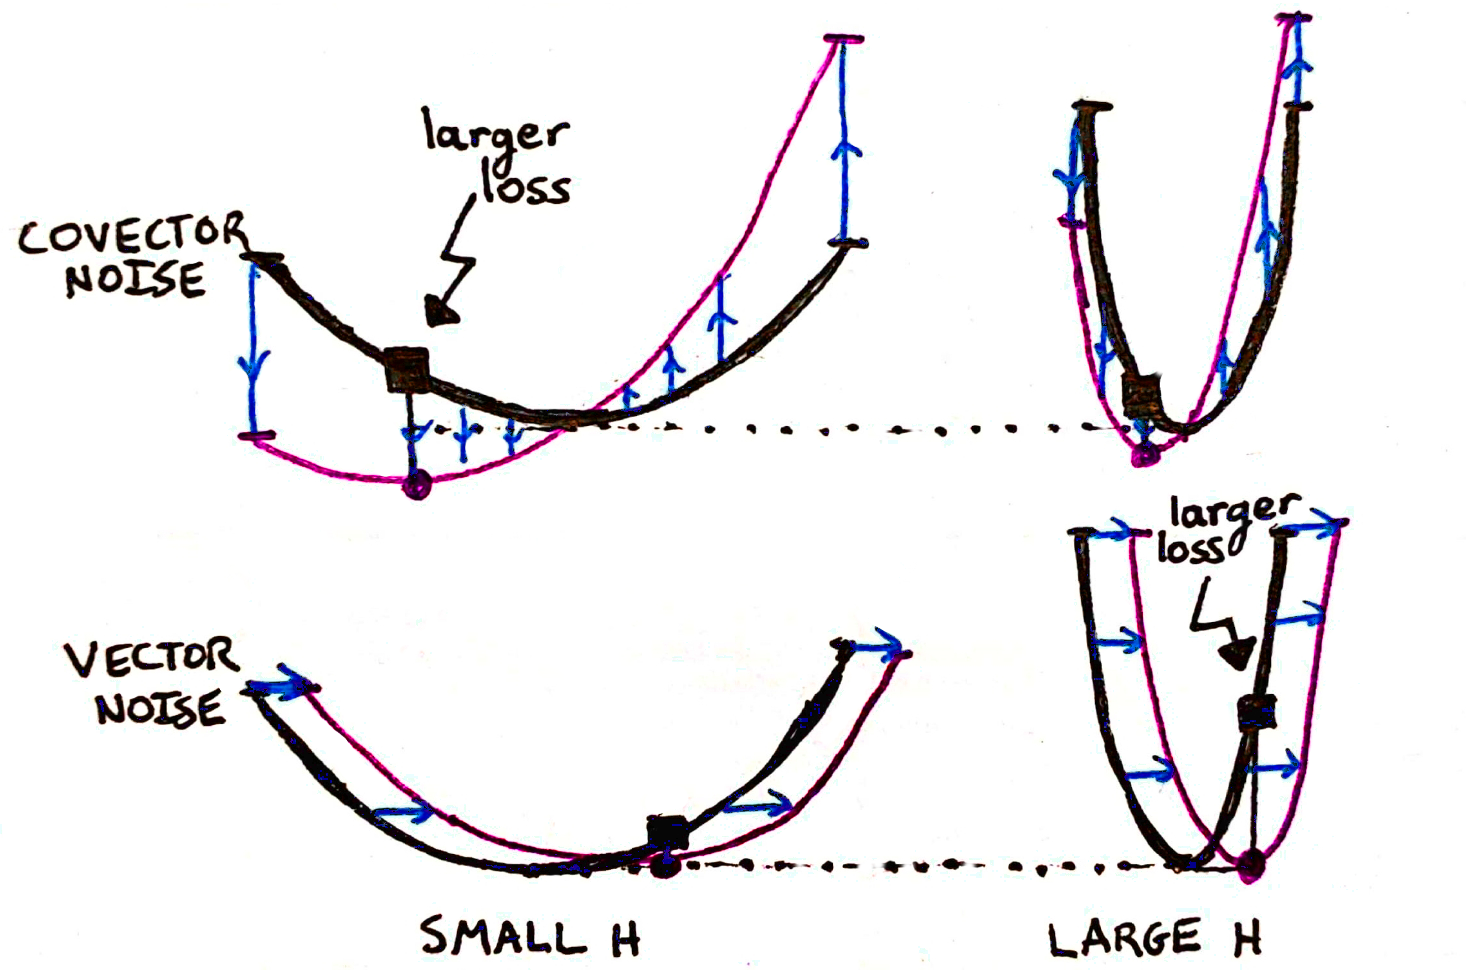
\includegraphics[width=0.49\linewidth, height=2cm]{../diagrams/sharp.png}
            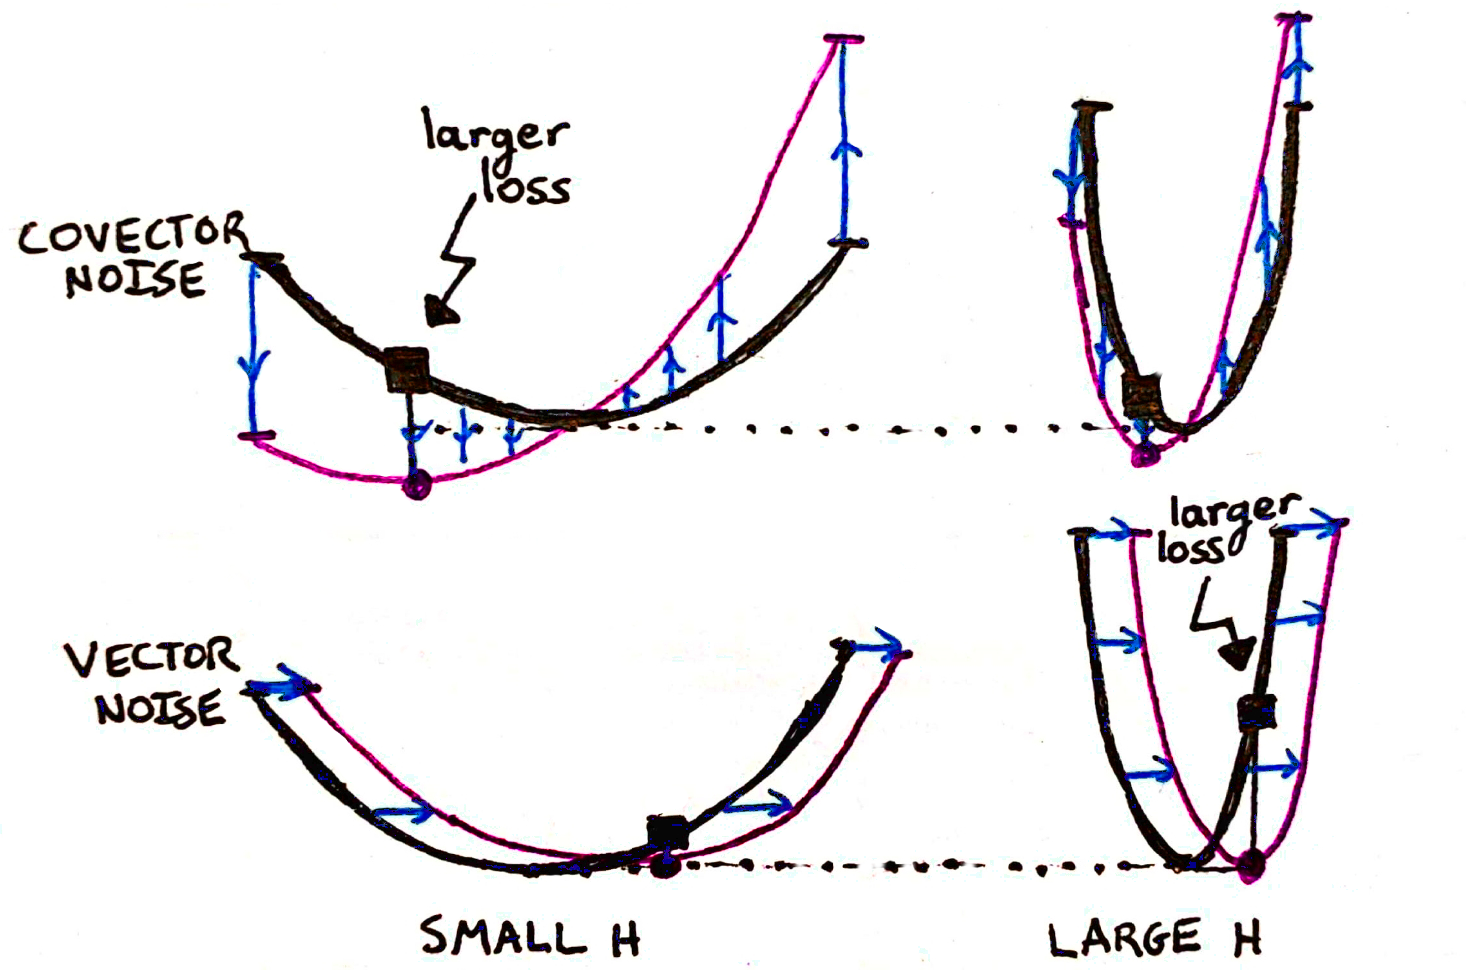
\includegraphics[width=0.49\linewidth, height=2cm]{../diagrams/sharp.png}
            \caption{Hi}
        \end{figure}



        The above generalizes \citet{ro18}'s $T=2$ result, proved without
        diagrams, to arbitrary $T$.  In principle, one could avoid diagrams
        completely by direct use of our Key Lemma.  However, as demonstrated by
        side-by-side comparison in the Appendix, the concept of counting
        concretizations of diagrams helps to streamline calculation, yielding
        arguments $4$ times shorter and arguably more insightful conceptual
        than direct perturbation.  The more complicated the computation, the
        greater the savings of using diagrams.

        %\begin{exm}
        %    We will encounter
        %    $$
        %        \sdia{(012-3)(03-13-23)}
        %            \triangleq
        %        \eta^3
        %        \expct{\nabla l_n} 
        %        \expct{\nabla l_n} 
        %        \expct{\nabla l_n} 
        %        \expct{\nabla\nabla\nabla l_n}
        %    $$
        %    as the leading contribution of non-gaussian noise to test loss.  
        %\end{exm}
        %\begin{exm}
        %    Diagrams whose rightmost node participates in a fuzzy ties
        %    contribute to train loss instead of test loss:
        %    $$
        %        \sdia{(02-13)(03-13-23)}
        %            \triangleq
        %        \eta^3
        %        \expct{\nabla l_n \nabla l_n} 
        %        \expct{\nabla l_n \nabla\nabla\nabla l_n}
        %    $$
        %\end{exm}

        %A final limitation we do not address in this work is that the  
        %expressions we derive are often expensive to compute.  Thus, we view
        %our main contributions as laying the foundations for a new type of
        %analysis.
        %
        %The more complicated the computation, the greater the savings of using
        %diagrams.

        %Amusing corollary about NP hardness of predicting final SGD location
        %after exponentially many steps.

    %    %-------------  illustration of diagrams embedded into spacetime  -----

    %    \begin{figure}[H] 
    %        \centering  
    %        \plotmooh{diagrams/spacetime-e}{}{0.265\columnwidth}
    %        \plotmooh{diagrams/spacetime-f}{}{0.265\columnwidth}
    %        \caption{
    %            {\bf Diagrams in spacetime dictate SGD's behavior.}  
    %            Some diagrams embedded in two spacetimes (grids of shaded
    %            cells) for $16$ steps on $8$ datapoints.  We arbitrarily choose
    %            colors to aid reference.  Nodes (here black) outside the grid
    %            represent a post-training measurement of test loss; their
    %            coordinates are arbitrary.
    %            {\bf Left}: SGD run with size-$1$ batches and 
    %                shuffling.  
    %                Reading across, we see:
    %                an illegal embedding of
    %                $\sdia{(01-2)(01-12)}$, a legal embedding of
    %                $\sdia{(01-2)(01-12)}$, and a legal embedding of
    %                $\sdia{(0-1-2)(01-12)}$.
    %                Since they have $4$ edges, they decay as $\eta^2$.   
    %            {\bf Right}: SGD run with size-$2$ batches and no
    %                shuffling.  Depicted is an embedding of a $4$-edged
    %                diagram, annotated with the data-weight interactions it
    %                represents.
    %                Since it has $4$ edges, it decays as $\eta^4$.   
    %                Section \ref{sect:calculus} gives numerical meaning
    %                to diagrams.  The
    %                test loss is a sum of infinitely many terms, each given
    %                by a different diagram embedding.  
    %        }
    %        \label{fig:spacetimes}
    %    \end{figure}

%==============================================================================
%=====  BACKGROUND AND NOTATION  ==============================================
%==============================================================================

\section{Background and Notation} \label{sect:background}

    %~~~~~~~~~~~~~~~~~~~~~~~~~~~~~~~~~~~~~~~~~~~~~~~~~~~~~~~~~~~~~~~~~~~~~~~~~~
    %~~~~~~~~~  The Loss Landscape  ~~~~~~~~~~~~~~~~~~~~~~~~~~~~~~~~~~~~~~~~~~~

    \subsection{The Loss Landscape}

        %-------------  review and defense of diagrams  -----------------------

        We henceforth fix a loss landscape on a weight space $\Mm$, i.e. a
        mean-$l$ distribution over smooth functions $l_n:\Mm\to\RR$.  We refer
        both to $n$ and to $l_n$ as \emph{datapoints}.

        %-------------  review and defense of diagrams  -----------------------

        More precisely, we fix a real-valued stochastic process indexed by the
        points of the \emph{weight space} $\Mm$, an affine manifold.  The
        process furnishes a \emph{train sequence} $(l_n: 0\leq n<N)$ of i.i.d.
        samples, each an unbiased estimate of $l$. We henceforth assume the
        regularity conditions listed in Appendix \ref{sect:proofs}, for
        instance that $l, l_n$ are analytic and that all moments exist.

        %-------------  specialization to a common case  ----------------------

        For example, these conditions admit $\tanh$ networks with cross entropy
        loss on bounded data --- and with arbitrary weight sharing, skip
        connections, soft attention, dropout, batch-normalization with disjoint
        batches, and weight decay.
        
    %~~~~~~~~~~~~~~~~~~~~~~~~~~~~~~~~~~~~~~~~~~~~~~~~~~~~~~~~~~~~~~~~~~~~~~~~~~
    %~~~~~~~~~  Tensor Conventions  ~~~~~~~~~~~~~~~~~~~~~~~~~~~~~~~~~~~~~~~~~~~

    \subsection{Tensor Conventions}
        We use $G_\mu, H_{\mu\nu}, J_{\mu\nu\lambda}$ for the first, second,
        and third derivatives of $l$ and $C_{\mu \nu}$ for the covariance of
        gradients.  By convention, our repeated Greek indices are implicitly
        summed: if $A_\mu, B^\mu$ are the coefficients of a covector $A$ and a
        vector
        $B$\footnote{
            Vectors/covectors are also called column/row vectors.
        }, indexed by basis elements $\mu$, then
        $
            A_\mu B^\mu
            \triangleq
            \sum_\mu A_\mu \cdot B^\mu
        $.
        To expedite dimensional analysis, we regard the learning rate as an
        inverse metric $\eta^{\mu\nu}$ that converts a gradient covector into a
        vector displacement \citep{bo13}.  We use $\eta$ to \emph{raise}
        indices.  In
        $
            H^{\mu}_{\lambda}
            \triangleq
            \eta^{\mu\nu} H_{\nu\lambda}
        $, for instance,
        $\eta$ raises one of $H_{\mu\nu}$'s indices.  Another example is
        $
            C^{\mu}_{\mu}
            \triangleq
            \sum_{\mu \nu} \eta^{\mu\nu} \cdot C_{\nu\mu}
        $.
        Standard syntactic constraints make manifest which expressions
        transform naturally with respect to optimization dynamics.  

        We say two expressions \emph{agree to order $\eta^d$} when
        their difference, divided by some homogeneous degree-$d$
        polynomial of $\eta$, tends to $0$ as $\eta$ shrinks.  Their
        difference is then $\in o(\eta^d)$.
        
    %~~~~~~~~~~~~~~~~~~~~~~~~~~~~~~~~~~~~~~~~~~~~~~~~~~~~~~~~~~~~~~~~~~~~~~~~~~
    %~~~~~~~~~  Names of SGD Parameters  ~~~~~~~~~~~~~~~~~~~~~~~~~~~~~~~~~~~~~~

    \subsection{SGD Terminology}
        SGD updates on the train sequence $(l_n: 0\leq n<N)$.
        For each of $M\cdot B$ \emph{epochs}, SGD partitions the $N$ datapoints
        into a length-$N/B$ sequence of size-$B$ \emph{batches}.  For each
        batch $\Bb$, SGD updates
        $
            \theta^\mu
            \leftsquigarrow
            \theta^\mu -
            \eta^{\mu\nu} \nabla_\nu
                \wrap{\frac{1}{B} \sum_{n\in \Bb} l_n(\theta)}
        $.
        SGD performs $N\cdot M$ many updates in total.  We write $l_t$ for the
        loss $\frac{1}{B}\sum_\Bb\cdots$ over the $t$th batch. 
        Together with an
        inter-epoch shuffling pattern, $N, B, M$ determine the SGD algorithm.
        The cases $B=1$ and $B=N$ we call \emph{pure SGD} and \emph{pure GD}.
        The $M=1$ case of pure SGD we call \emph{vanilla SGD}.

    \subsection{Diagrams and Embeddings}

%==============================================================================
%=====  DIAGRAM CALCULUS FOR SGD  =============================================
%==============================================================================

\section{Diagram Calculus for SGD} \label{sect:calculus}

    %~~~~~~~~~~~~~~~~~~~~~~~~~~~~~~~~~~~~~~~~~~~~~~~~~~~~~~~~~~~~~~~~~~~~~~~~~~
    %~~~~~~~~~  Role of Diagrams  ~~~~~~~~~~~~~~~~~~~~~~~~~~~~~~~~~~~~~~~~~~~~~

    \subsection{How Diagrams Arise}

        Suppose $s$ is analytic on weight space, for example $s=l$.
        We track $s(\theta)$ as SGD updates $\theta$: %(c.f. \citet{dy49a}):
        \begin{klem*} %\label{lem:dyson}
            For all $T$: for $\eta$ sufficiently small, $s(\theta_T)$ is
            \begin{equation}\label{eq:dyson}
                \sum_{(d_t: 0\leq t<T)}
                (-\eta)^{\sum_t d_t}
                \left(
                    \prod_{0 \leq t < T}
                        \left.
                            \frac{(g \nabla)^{d_t}}{d_t!}
                        \right|_{g={\color{moor}\nabla l_t(\theta)}}
                \right)
                (s) (\theta_0)
            \end{equation}
            Moreover, the expectation symbol (over train sets) commutes with
            the sum over $d$s.
        \end{klem*}
        In averaging over train sets we may factor the expectation of the above
        product according to independence relations between the $l_t$.  We view
        various training procedures (e.g. pure GD, pure SGD) as
        \emph{prescribing different independence relations} that lead to
        different factorizations and hence to potentially different
        generalization behavior at each order.
    
        An instance of the above product (for $s=l_a$ drawn from a test set and
        $0\leq c\leq b<T$) is $-\eta^3 (\nabla l_c \nabla)^2 (\nabla l_b
        \nabla) l_a$, which is
        {\small
        \begin{align*}
            - (\nabla^\lambda l_c) (\nabla^\mu l_c) (\nabla_\lambda \nabla_\mu \nabla^\nu l_b) (\nabla_\nu l_a)   
            - (\nabla^\lambda l_c) (\nabla^\mu l_c) (\nabla_\lambda \nabla^\nu l_b) (\nabla_\mu \nabla_\nu l_a) \\
            - (\nabla^\lambda l_c) (\nabla^\mu l_c) (\nabla_\mu \nabla^\nu l_b) (\nabla_\lambda \nabla_\nu l_a)   
            - (\nabla^\lambda l_c) (\nabla^\mu l_c) (\nabla^\nu l_b) (\nabla_\lambda \nabla_\mu \nabla_\nu l_a)
        \end{align*}
        }
        To reduce clutter, we draw contractions as thin edges and datapoint
        equalities as fuzzy ties\footnote{This visual scheme echoes
        \citet{fe49, pe71}.}.  Then, in expectation over
        $(l_c, l_b, l_a)$ drawn i.i.d.:
        \begin{align}
            \cdots
            &= 
                 \sdia{(01-2-3)(02-12-23)}
                +\sdia{(01-2-3)(02-13-23)}
                +\sdia{(01-2-3)(03-12-23)}
                +\sdia{(01-2-3)(03-13-23)} \\
                \label{eq:simpl}
            &=
                \underbrace{2\sdia{(01-2-3)(02-12-23)}}_{
                   -2~\expct{{\color{moor}(\nabla l)(\nabla l)}}~\expct{{\color{moog}\nabla\nabla\nabla l}}~\expct{{\color{moob} \nabla l}}
                }
                +
                \underbrace{2\sdia{(01-2-3)(02-13-23)}}_{
                   -2~\expct{{\color{moor}(\nabla l)(\nabla l)}}~\expct{{\color{moog}\nabla \nabla l}}~\expct{{\color{moob}\nabla \nabla l}}
                }
        \end{align}
        Each degree-$g$ node corresponds to an $l_n$ (here,
            {\color{moor} $l_c$},
            {\color{moog} $l_b$},
            {\color{moob} $l_a$}) differentiated $g$ times
        (for instance, {\color{moog} $l_b$} is differentiated thrice in the
        first diagram and twice in the second).  Thin \emph{edges} mark
        contractions by $-\eta$.  Fuzzy \emph{ties} denote correlations by
        connecting identical loss functions (here, {\color{moor} $l_c$} with
        {\color{moor} $l_c$}), and are visually emphasized by otherwise
        meaningless colors.
        \begin{defn}
            A diagram $D$ evaluates to the expected value
            $\dvalue(D)$ of the corresponding tensor expression.
        \end{defn}
        % 
        Usefully, % for a fixed, i.i.d.  distribution over $(l_c, l_b, l_a)$,
        \emph{the topology of a diagram determines its value}.  For instance,
        simplification \ref{eq:simpl} is licensed because
        $
            \dvalue\wrap{\sdia{(01-2-3)(02-12-23)}}
            =
            \dvalue\wrap{\sdia{(01-2-3)(03-13-23)}}
        $.
        We will sometimes write a diagram $D$ and mean $\dvalue(D)$. 
    
        \begin{defn}[Fuzzy Outlines Denote Noise's Net Effect]
            So, if $D$ is a diagram and $p, \tilde p$ are two parts of $D$'s
            parition, let $D_{p\tilde p}$ be the diagram with $p, \tilde p$
            joined into a single part.  So:
            $
                (\sdia{(0-1)(01)})_{\text{\color{moor}red}~\text{\color{moog}green}}
                \triangleq
                \sdia{(01)(01)}
            $
            and
            $
                (\sdia{(01-2-3)(02-12-23)})_{\text{\color{moor}red}~\text{\color{moob}blue}}
                \triangleq
                \sdia{(013-2)(02-12-23)}
            $.
            Differences such as $D_{p\tilde p}-D$ will often concern us, so we
            define a diagram with fuzzy \emph{outlines} to represent the
            difference between the fuzzy tied and untied versions so that
            $
                \sdia{c(0-12)(01-12)}
                \triangleq
                (\sdia{(0-1-2)(01-12)})_{\text{\color{moog}green}~\text{\color{moob}blue}}
                -
                \sdia{(0-1-2)(01-12)}
                =
                \sdia{(0-12)(01-12)}
                -
                \sdia{(0-1-2)(01-12)}
            $.
        \end{defn}

    %~~~~~~~~~~~~~~~~~~~~~~~~~~~~~~~~~~~~~~~~~~~~~~~~~~~~~~~~~~~~~~~~~~~~~~~~~~
    %~~~~~~~~~  Recipe for Test Loss and Generalization Gap  ~~~~~~~~~~~~~~~~~~
           
    \subsection{Recipe for SGD's Test Loss and Generalization}

        Our main tool, proved in Appendix \ref{sect:proofs}, follows.
        
        \begin{thm}[Test Loss as a Path Integral] \label{thm:sgdcoef}
            For all $T$: for $\eta$ sufficiently small, SGD's expected test
            loss is
            \begin{equation*}\label{eq:sgdcoef}
                \sum_{D \in \image(\Free)} \wrap{
                    \sum_{f: D\to\Free(S)}
                    \frac{1}{\wabs{\Aut_f(D)}}
                }
                \frac{\dvalue(D)}{B^{|\edges(D)|}}
            \end{equation*}
            Here, $D$ is a diagram whose root $r$ participates in no fuzzy
            edge,    $f$ represents an embedding of $D$ into spacetime, and
            $\wabs{\Aut_f(D)}$ counts the graph-automorphisms of $D$ that
            preserve $f$'s assignment of nodes to cells.
            %
            Replacing each $\dvalue(D)$ by
            $
                \wrap{-\sum_{p \in \parts(D)} \dvalue(D_{rp} - D)/N}
            $,
            we obtain the expected generalization gap (test minus train
            loss).
        \end{thm}
    
        \begin{prop}[Specialization to Vanilla SGD] \label{prop:vanilla}
            The order $\eta^d$ contribution to the expected test loss of
            one-epoch SGD with singleton batches is:
            \begin{equation*}\label{eq:sgdbasiccoef}
                \frac{(-1)^d}{d!} \sum_{D\in \image(\Free)} 
                |\ords(D)| {N \choose P-1} {d \choose d_0,\cdots,d_{P-1}}
                \dvalue(D)
            \end{equation*}
            where $D$ ranges over $d$-edged diagrams whose equivalence classes
            have sizes $d_p: 0\leq p\leq P$, with $d_P=1$
            and, without loss, are each antichains.  The modification to
            compute the generalization gap is the same as in Theorem
            \ref{thm:sgdcoef}.
        \end{prop}
        \begin{rmk}[Vanilla SGD's Deviation from ODE] \label{rmk:vsode}
            A $P$-part, $d$-edged diagram contributes $\Theta\left((\eta N)^d
            N^{P-d-1}\right)$ to the loss.  For example, there are $6$ diagrams
            to order $3$, and they have $(4+2)+(2+2+3)+(1)$ many orderings (see
            Table \ref{tab:scatthree}).  Intuitively, $\eta N$ measures the
            physical time of descent and $1/N$ measures the coarseness of time
            discretization.  Thus arises a double-series in $(\eta N)^d
            N^{P-d-1}$, where $d$ counts thin edges and $d+1-P$ counts fuzzy
            ties; the $P=d+1$ terms correspond to a noiseless,
            discretization-agnostic (hence ODE) approximation to SGD, while
            $P\leq d$ gives correction terms modeling time-discretization and
            noise.  
        \end{rmk}

    \subsection{Consequences of the Recipe}

        %~~~~~~~~~~~~~~~~~~~~~~~~~~~~~~~~~~~~~~~~~~~~~~~~~~~~~~~~~~~~~~~~~~~~~~
        %~~~~~  Theoretical Corollaries  ~~~~~~~~~~~~~~~~~~~~~~~~~~~~~~~~~~~~~~

        For accessibility, we write our results with Greek indices instead of
        diagrams.  However, as Appendices \ref{sect:tutorial},
        \ref{sect:compare}, and \ref{sect:calculations} show, diagrams are
        crucial for proving --- and for identifying the data-weight processes
        that govern --- these results.

        \begin{cor}[SGD Differs from ODE and SDE] \label{cor:vsode}
            The test loss of vanilla SGD deviates at order $N^{-1}$ from
            ODE by
            $
                \frac{T^2 N^{-1}}{2} ~ C_{\mu\nu} H^{\mu\nu}
            $.
            Its order $N^{-2}$ deviation due to non-Gaussian noise is
            $
                \frac{T^3 N^{-2}}{6} \wrap{
                    \sdia{c(012-3)(03-13-23)}
                    -
                    3 \sdia{c(01-2-3)(03-13-23)}
                }
                =
                -
                \frac{T^3 N^{-2}}{6}  
                \wrap{
                    \wrap{
                        \expct{\nabla_\mu l_x \nabla_\nu l_x \nabla_\lambda l_x}-
                        G_\mu G_\nu G_\lambda
                    }
                    J^{\mu\nu\lambda}
                    - 
                    3
                    C_{\mu \nu} G_\lambda J^{\mu\nu\lambda}
                }
            $.
            These effects contribute to SGD's difference from SDE.
        \end{cor}
        For finite $N$, these effects separate SDE from SGD.  SDE also fails to
        model multi-epoch SGD's inter-update correlations.  Conversely, as
        $N\to\infty$ so that SDE matches SGD, optimization and generalization
        respectively become computationally intractable and trivial and hence
        less interesting.
    
        \begin{table}[h]
            \centering 
            \resizebox{\columnwidth}{!}{%
            \begin{tabular}{c|c|c}
                {\LARGE $\Theta\left((\eta N)^3 N^{-0}\right)$} &
                {\LARGE $\Theta\left((\eta N)^3 N^{-1}\right)$} &
                {\LARGE $\Theta\left((\eta N)^3 N^{-2}\right)$} \\ \hline
                \begin{tabular}{c}
                    \begin{tabular}{LL}
                        \bdia{(0-1-2-3)(01-12-23)} & \bdia{(0-1-2-3)(01-13-23)}
                    \end{tabular} \\
                    \begin{tabular}{LL}
                        \bdia{(0-1-2-3)(02-13-23)} & \bdia{(0-1-2-3)(03-12-23)}
                    \end{tabular} \\ \hline
                    \begin{tabular}{LL}
                        \bdia{(0-1-2-3)(03-13-23)} & \bdia{(0-1-2-3)(02-12-23)}
                    \end{tabular}
                \end{tabular}
                &
                \begin{tabular}{c}
                    \begin{tabular}{LL}
                        \bdia{(01-2-3)(02-13-23)} & \bdia{(01-2-3)(03-12-23)}
                    \end{tabular} \\ \hline
                    \begin{tabular}{LL}
                        \bdia{(0-12-3)(01-13-23)} & \bdia{(0-12-3)(02-13-23)}
                    \end{tabular} \\ \hline
                    \begin{tabular}{LLL}
                        \bdia{(01-2-3)(03-13-23)} & \bdia{(0-12-3)(03-13-23)} & \bdia{(01-2-3)(02-12-23)} 
                    \end{tabular}
                \end{tabular}
                &
                \begin{tabular}{c}
                    \begin{tabular}{L}
                        \bdia{(012-3)(03-13-23)}
                    \end{tabular}
                \end{tabular}
            \end{tabular}
            }
            \caption{
                Degree-$3$ scattering diagrams for $B=M=1$ SGD's test loss.
                {\bf Left:} $(d, P) = (3, 3)$.  Diagrams for ODE behavior.
                {\bf Center:} $(d, P) = (3, 2)$.  $1$st order deviation of SGD
                away from ODE.
                {\bf Right:} $(d, P) = (3, 1)$.  $2$nd order deviation of SGD
                from ODE with appearance of non-Gaussian statistics.
            }
            \label{tab:scatthree}
        \end{table}
    
        \begin{cor}[Shuffling Barely Matters] \label{cor:shuffle}
            To order $\eta^3$, inter-epoch shuffling doesn't affect SGD's
            expected test loss.
        \end{cor}
        Indeed, for any inter-epoch shuffling scheme: 
        \begin{prop}\label{prop:ordtwo}
            To order $\eta^2$, the test loss of SGD --- on $N$
            samples for $M$ epochs with batch size $B$ dividing $N$ and with any
            shuffling scheme --- has expectation
            {\small
            \begin{align*}
                                                        l              
                &- MN                                   G_\mu G^\mu       
                 + MN\wrap{MN - \frac{1}{2}}            G_\mu H^{\mu}_{\nu} G^\nu \\
                &+ MN\wrap{\frac{M}{2}}                 C_{\mu \nu} H^{\mu \nu}
                 + MN\wrap{\frac{M-\frac{1}{B}}{2}}     \wrap{\nabla_\mu C^{\nu}_{\nu}} G^\mu / 2
            \end{align*}
            }
        \end{prop}
    
        \begin{cor}[The Effect of Epoch Number] \label{cor:epochs}
            To order $\eta^2$, one-epoch SGD has 
            $
                 \wrap{\frac{M-1}{M}}\wrap{\frac{B+1}{B}}\wrap{\frac{N}{2}}
                 \wrap{\nabla_\mu C^{\nu}_{\nu}} G^\mu / 2
            $
            less test loss than $M$-epoch SGD with learning rate $\eta/M$.
        \end{cor}
    
        Upon analyzing $\sdia{c(01-2)(01-12)}$: given a smooth unbiased
        estimator $\hat{C}$ of gradient covariance, we may cause GD to mimic
        SGD:
        \begin{cor}[The Effect of Batch Size] \label{cor:batch}
            The expected test loss of pure SGD is, to order $\eta^2$,
            less than that of pure GD by
            $
                  \frac{M(N-1)}{2} ~
                  \wrap{\nabla_\mu C^{\nu}_{\nu}} G^\mu / 2
            $.
            Moreover, GD on a modified loss 
            $
                \tilde l_n = l_n +
                    \frac{N-1}{4N} ~
                    \hat{C}_\nu^\nu(\theta)
            $
            has an expected test loss that agrees with SGD's to second order.
            We call this method GDC.
        \end{cor}
    
        \begin{cor}[An Entropic Force, Unrenormalized] \label{cor:noncons}
            When vanilla SGD is initialized at a test minimum, the weight is
            displaced to order $\eta^3$ by 
            $
                -{T \choose 2} C_{\mu \nu} J^{\mu \nu \lambda}
            $.
        \end{cor}
        Corollary \ref{cor:noncons} was first proven by \citet{ya19b}; our
        methods reproduce it elegantly.  We will renormalize it to Corollary
        \ref{cor:entropic}, which applies for large times, hence demonstrating
        a persistent and non-conservative entropic force.
    
    %--------------------------------------------------------------------------
    %           Toward Effective Theories                   
    %--------------------------------------------------------------------------

    \subsection{Effective Theories} \label{subsect:effective}
        The mathematics of \emph{renormalization} summarizes myriad small-scale
        interactions into an effective large-scale theory.  We will renormalize
        by pairing diagrams of interest with topologically related diagrams in
        order to refine our $d$th order estimates for any fixed $d$.  In some
        large-$\eta T$ settings, the unrenormalized theory does not converge
        while the renormalized theory does.  Thus, renormalization will help us
        reason about large-time behavior. 

        As a motivating example, consider that, to order $\eta^1$, SGD reduces
        test loss by $T G_\mu G^\mu$ (c.f. \citet{ne04}).  Though useful for
        small $\eta T$, this approximation diverges as $T$ grows.  Intuitively,
        the this approximation suffers because it does not account for evolving
        gradients, i.e.  for the Hessian.  Let us thus consider the diagrams
        that are uncorrelated chains:
        $
            \sdia{(0-1)(01)}, \sdia{(0-1-2)(01-12)},
            \sdia{(0-1-2-3)(01-12-23)}, \cdots
        $.  This infinite sequence epitomizes the effect of the Hessian
        (degree $2$ nodes).
        When embedded with initial and final nodes separated by duration
        $\Delta t$, this series of diagrams sums to
        $
            -G (I-\eta H)^{\Delta t-1} \eta G
            \approx
            -G \exp(-\eta \Delta t H) \eta G
            \cdot (1+o(\eta))
        $.
        The $\exp(-\eta \Delta t H) \eta$ is thus an ``effective learning
        rate'' to be used in place of $\eta$ in renormalized calculations.
        Summed over all embeddings, the above chains contribute $G \sum_{0\leq
        t<T} (I-\eta H)^{T-t-1} \eta G$ to vanilla SGD's test loss, or:
        \begin{align*}
            \approx
            -G \wrap{\int_t \exp(-\eta (T-t) H)} \eta G
            =
            -G \wrap{\frac{I - \exp(-\eta T H)}{H}} G
        \end{align*}
        In contrast to the unrenormalized prediction $T G_\mu G^\mu$,
        the above converges in the large-$T$ limit (when $H$ is positive).

        So the chains form a class of diagrams usefully analyzed
        together.  We may likewise organize other diagrams.  We will
        represent each class by its minimal element:
        \begin{defn}
            A diagram is \emph{irreducible} when it lacks non-root
            un-fuzzily-tied degree-two nodes (such as $\sdia{(0-1-2)(01-12)}$'s
            {\color{moog}green} node).
            So
            $\sdia{(0-1-2)(02-12)}$ and
            $\sdia{(01-2)(01-12)}$
            but neither
            $\sdia{(0-1-2)(01-12)}$ nor
            $\sdia{(02-1-3)(01-12-23)}$
            are irreducible.
        \end{defn}

        \begin{defn}[Embedding-Sensitive Values]
            \label{defn:rvalue}
            Let $\rvalue_f(D)$ be the expected value of $D$'s corresponding
            tensor expression, where instead of using $-\eta$ to contract
            two tensors embedded to times $t, t+\Delta t$, we use
            $
                -(I-\eta H)^{\Delta t - 1} \eta
            $.
            Actually, as we study the effect of noise, it will be most
            convenient to let $\rvalue$s represent a \emph{difference} from the
            noiseless case.  For the small diagrams we consider, we obtain
            $\rvalue$s by replacing fuzzy ties by fuzzy outlines; larger
            diagrams present complications addressed in
            Appendix \ref{subsubsect:mobius}.
        \end{defn}

        \textsc{Renormalized Recipe:}~
            In general, one sums over embeddings of irreducible diagrams, using
            $\rvalue_f(D)$ instead of $\dvalue(D)$.  In practice, we prefer to
            approximate sums over embeddings by integrals over times and
            $(I-\eta H)^t$ by $\exp(- \eta H t)$, hence incurring a
            term-by-term multiplicative error of $1 + o(\eta)$ that preserves
            leading order results.  Diagrams thus induce easily evaluated
            integrals of exponentials.
       
        \begin{thm}[Renormalization Gives Large-$T$ Limits] \label{thm:renorm}
            For any $T$: for $\eta$ sufficiently small, SGD's expected test
            loss exceeds the noiseless case by 
            \begin{equation*} \label{eq:renorm}
                \sum_{\substack{
                    D \in \image(\Free)\\ \text{\color{moor} irreducible}
                }}
                \wrap{
                    \sum_{f: D\to\Free(S)}
                    \frac{1}{\wabs{\Aut_f(D)}}
                }
                \frac{{\color{moor} \rvalue_f}(D)}{B^{|\edges(D)|}}
            \end{equation*}
            In contrast to Theorem \ref{thm:sgdcoef}: when $H$ is positive, the
            $d$th order truncation converges as $T$ diverges.
        \end{thm}
        That convergence property formally licenses long-term limits of
        renormalized predictions.  In fact, the convergence is uniform in $T$
        for sufficiently regular landscapes.

        \begin{figure}[h!]
            \centering  
            \plotmooh{diagrams/spacetime-g}{}{0.210\columnwidth}
            \plotmooh{diagrams/spacetime-h}{}{0.210\columnwidth}
            \caption{
                {\bf Renormalization summarizes Hessians' long-term effect.}
                {\bf Left}:
                    Some contributions to $\rvalue_f(\sdia{(0-1)(01)})$ for an
                    example embedding $f$.  Theorem \ref{thm:renorm} shows how
                    (geometric series) and why (improved convergence) we
                    consider these diagrams as a group.
                {\bf Right}:
                    A contribution to $\rvalue_f(\sdia{(01-2)(02-12)})$.  The
                    leftmost {\color{mooteal}teal} nodes depict a disturbance
                    by noise (multi-node cells or rows correspond higher
                    moments and hence to noise).  The noise travels through two
                    channels (top, bottom) before interacting with the test
                    Hessian (degree-two black node).  Such embeddings give the
                    small-$\eta$, large-$T$ interaction of noise and curvature. 
                {\bf Both}:
                    In violation of our rule for valid embeddings, the nodes
                    inserted into the irreducible diagrams may occupy the same
                    row despite lacking fuzzy ties.  Overcounting
                    accompanies our $(I-\eta H)^{\Delta t-1}$ prescription; it
                    is countered as described Appendix \ref{subsubsect:mobius}
                    and implicit in Theorem \ref{thm:renorm}.
            }
            \label{fig:renormspacetime}
        \end{figure}

        Integrating $\rvalue_f(\sdia{(01-2-3)(02-12-23)})$ over embeddings $f$, we see:
        \begin{cor}[A Nonconservative Entropic Force]\label{cor:entropic}
            Initialized at a test minimum, vanilla SGD's weight moves to
            order $\eta^2$ with a long-time-averaged\footnote{
                That is, $T$ so large that $C \exp(-\eta K T)$ is negligible.
                Appendix \ref{sect:calculations} gives a similar expression for general $T$.
            }
            expected velocity of
            $$
                v^\pi = C_{\mu \nu}
                \wrap{K^{-1}}^{\mu\nu}_{\rho\lambda}
                J^{\rho\lambda}_{\sigma}
                \wrap{\frac{I - \exp(-T \eta H)}{T \eta H} \eta}^{\sigma \pi}
            $$
            per timestep.
            Here, $K = \eta H \otimes I + I \otimes \eta H$, a
            $4$-valent tensor. 
        \end{cor}
        Unlike \citet{we19b}, we make no assumptions of thermal equilibrium,
        fast-slow mode separation, or constant covariance.  This generality
        reveals a novel, empirically verified dynamical phenomenon, namely that
        the velocity field above need not be conservative.

        Integrating $\rvalue_f(\sdia{(01-2)(02-12)})$ and
        $\rvalue_f(\sdia{(01)(01)})$ yields:
        \begin{cor}[Flat, Sharp Minima Overfit Less]\label{cor:overfit}
            Initialized at a test minimum, pure GD's test loss is to
            order $\eta$
            $$
                \frac{1}{2N} ~
                    C_{\mu\nu}
                    \wrap{(I - \exp(-\eta T H))^{\otimes 2}}^{\mu\nu}_{\rho\lambda}
                    \wrap{H^{-1}}^{\rho\lambda}
            $$
            above the minimum.  This vanishes when $H$ does. 
            Likewise, pure GD's generalization gap is to order $\eta$:  
            $$
                \frac{1}{N} ~
                    C_{\mu\nu}
                    \wrap{I - \exp(-\eta T H)}^{\nu}_{\lambda}
                    \wrap{H^{-1}}^{\lambda\mu}
            $$
            In contrast to the later-mentioned Takeuchi estimate, this does not
            diverge as $H$ shrinks.
        \end{cor}
        Corollary \ref{cor:overfit}'s generalization gap converges after large
        $T$ to $C_{\mu\nu}(H^{-1})^{\mu\nu}/N$, also known as Takeuchi's
        Information Criterion (TIC).  In turn, in the classical setting of
        maximum likelihood (ML) estimation (with no model misspecification)
        near the ``true'' test minimum, $C=H$ is the Fisher metric, so we
        recover AIC $(\textnormal{number of parameters})/N$.  Unlike AIC, our
        more general expression is descendably smooth, may be used with MAP or
        ELBO tasks instead of just ML, and makes no model well-specification
        assumptions.

        \begin{figure}[h!]
            \centering
            \plotmooh{diagrams/entropic-force-diagram}{}{0.32\columnwidth} 
            \plotmooh{diagrams/sharp}{}{0.31\columnwidth}
            \caption{
                {\bf Renormalization reveals novel phenomena
                with physical interpretations.}
                {\bf Left}:
                    The entropic force mechanism: gradient noise induces a flow
                    toward minima flat \emph{with respect to to the
                    covariance}.  Although our analysis assumes neither thermal
                    equilibrium nor fast-slow mode separation, we label ``fast
                    and slow directions'' in this figure to ease comparison
                    with \citet{we19b}.  In this figure, red densities denote
                    the spread predicted by a renormalized $C^{\mu\nu}$, and
                    the spatial variation of curvature corresponds to
                    $J_{\mu\nu\lambda}$. 
                {\bf Right}:
                    Noise structure determines how curvature affects
                    overfitting.  To use a physical metaphor, for a fixed
                    displacement scale, stiffer springs incur greater energy
                    gains.  But for a fixed force scale, limper springs incur
                    greater energy gains.  Geometrically, for (empirical risk
                    minimization on) a vector-perturbed landscape, small
                    Hessians are favored (top row), while for
                    covector-perturbed, landscape large Hessians are favored
                    (bottom row).  Corollary \ref{cor:overfit} shows how the
                    implicit regularization of fixed-$\eta T$ descent mediates
                    between the two rows.
            }
            \label{fig:cubicandspring}
        \end{figure}

%==============================================================================
%    EXPERIMENTS AND APPLICATIONS
%==============================================================================

\section{Experiments}

    We focus on experiments whose rejection of the null hypothesis (and hence
    support of our theory) is so drastic as to be visually obvious.  For
    example, in Figure \ref{fig:thermoandtak}, \citep{ch18} predicts a velocity
    of $0$ while we predict a velocity of $\eta^2/6$.  
    %
    Throughout, \texttt{I} bars and \texttt{+} marks denote a 95\% confidence
    interval based on the standard error of the mean, in the vertical or
    vertical-and-horizontal directions, respectively.  See Appendix
    \ref{sect:landscape} for experimental procedure including architectures and
    sample size.

    %--------------------------------------------------------------------------
    %           Vanilla SGD; Epochs and Overfitting         
    %--------------------------------------------------------------------------

    \subsection{Basic Predictions}
        We test Proposition \ref{prop:vanilla} by direct measurement of smooth
        convnets on CIFAR-10 and Fashion-MNIST.  Our order $\eta^3$
        perturbative predictions up to $\eta T \approx 10^0$ (Figure
        \ref{fig:vanillaandbatch}, left).  Likewise, Corollary \ref{cor:epochs}
        predictions about epochs agree with experiment (Appendix
        \ref{sect:figures}).  These tests verify that the Proposition
        hides no mistakes of proportionality or sign.  

    %--------------------------------------------------------------------------
    %           Emulating Small Batches with Large Ones     
    %--------------------------------------------------------------------------

    \subsection{Emulating Small Batches with Large Ones}
        Figure \ref{fig:vanillaandbatch} (right) shows that the regularizer
        proposed in Corollary \ref{cor:batch} indeed enables GD to emulate SGD
        on a range of image-classification landscapes.  For these experiments,
        we used a covariance estimator $\hat C \propto \nabla l_x (\nabla l_x -
        \nabla l_y)$ evaluated on two batches $x, y$ that evenly partition the
        train set.  For architectures composed of linear transforms and
        coordinate-wise nonlinearities represented by elementary functions, we
        may compute $\nabla \hat C$ with the same memory and time as the usual
        gradient $\nabla l_t$, up to a multiplicative constant. 
        \begin{figure}[h!] 
            \centering
            \plotmoow{plots/new-test-0}{0.48\columnwidth}{3.0cm} 
            \plotmoow{plots/new-big-bm-new}{0.48\columnwidth}{4.0cm}
            \caption{
                {\bf Perturbation models SGD and GD.}
                {\bf Left}: Test loss vs learning rate on a Fashion-MNIST
                convnet.  For the instance shown and all $11$ other
                initializations unshown, the degree-$3$ prediction agrees with
                experiment through $\eta T \approx 10^0$.
                %
                {\bf Right}: with equal-scaled axes, this plot shows that GDC
                matches SGD (small vertical variation) better than GD matches
                SGD (large horizontal variation) in test loss, for a variety of
                learning rates (from 0.0025 to 0.1) and initializations (zero
                and multiple independent Xavier-Glorot trials) on several of
                image classification landscapes (logistic and convolutional
                CIFAR-10 and Fashion-MNIST).  $T=10$ throughout.
            }
            \label{fig:vanillaandbatch}
        \end{figure}
  
    %--------------------------------------------------------------------------
    %           Comparison to Continuous Time               
    %--------------------------------------------------------------------------

    \subsection{Comparison to Continuous Time} \label{subsect:gaussfit}
        Consider fitting a centered normal $\Nn(0, \sigma^2)$ to some centered
        standard normal data.  We parameterize the landscape by
        $h=\log(\sigma^2)$ so that the Fisher information matches the standard
        dot product \citep{am98}.  The gradient at sample $x$ and weight
        $\sigma$ is then $g_x(h) = (1-x^2\exp(-h))/2$.  Since $x\sim \Nn(0,
        1)$, $g_x(h)$ will be affinely related to a chi-squared, and in
        particular non-Gaussian.  At $h=0$, the expected gradient vanishes, and
        the test loss of vanilla SGD only involves diagrams with no singleton
        leaves; to third order, it is
        $
            \sdia{(0)()}
            +\frac{T}{2} \sdia{c(01-2)(02-12)}
            +{T\choose 2} \sdia{c(03-1-2)(01-12-23)}
            +\frac{T}{6} \sdia{c(012-3)(03-13-23)}
        $
        In particular, the ${T\choose 2}$ differs from $T^2/2$ and hence
        contributes to the time-discretization error of SDE as an approximation
        for SDE.  Moreover, non-Gaussian noise contributes via
        $\sdia{c(012-3)(03-13-23)}$ to that error.  Appendix \ref{sect:figures}
        shows that SDE and one-epoch SGD indeed differ.  For multi-epoch
        SGD, the effect of overfitting to finite training data further
        separates SDE and SGD.

    %--------------------------------------------------------------------------
    %           Thermodynamic Engine                        
    %--------------------------------------------------------------------------

    \subsection{A Nonconservative Entropic Force} \label{subsect:entropic}
        To test Corollary \ref{cor:entropic}'s predicted force, we construct a
        counter-intuitive loss landscape wherein, for arbitrarily small
        learning rates, SGD steadily increases the weight's z component despite
        0 test gradient in that direction.  Our mechanism differs from that
        discovered by \citet{ch18}.  Specifically, because in this landscape
        the force is $\eta$-perpendicular to the image of $\eta C$, that work
        predicts an entropic force of $0$.  This disagreement in predictions is
        possible because our analysis does not make any assumptions of
        equilibrium, conservatism, or continuous time.

        Intuitively, the presence of the term
        $
            \sdia{c(01-2-3)(02-12-23)}
        $
        in our test loss expansion indicates that \emph{SGD descends on a
        covariance-smoothed landscape}.  So, even in a valley of global minima,
        SGD will move away from minima whose Hessian aligns with the current
        covariance.  However, by the time it moves, the new covariance might
        differ from the old one, and SGD will be repelled by different Hessians
        than before.  Setting the covariance to lag the Hessian by a phase, we
        construct a landscape in which this entropic force dominates.  This
        ``\emph{linear screw}'' landscape has
        %
        $3$-dimensional $w\in \RR^3$ (initialized to $0$) and
        %
        $1$-dimensional $x \sim \Nn(0, 1)$:
        $$
            l_x(w)
            \triangleq
            \frac{1}{2} H(z)(w, w) + x \cdot S(z)(w)  
        $$
        Here, $H(z)(w, w) = w_x^2 + w_y^2 + (\cos(z) w_x + \sin(z) w_y)^2$
        %
        and   $S(z)(w)    = \cos(z-\pi/4) w_x + \sin(z-\pi/4) w_y$.
        %
        We see that there is a valley of global minima defined by $x=y=0$. 
        If SGD is initialized there, then to leading order in $\eta$ and for
        large $T$, the renormalized theory predicts a $z$-speed of $\eta^2/6$ 
        per timestep.  Upon renormalization, our predictions thus agree for
        large $\eta T$ with experiment (Figure \ref{fig:thermoandtak}, left).

        By stitching together copies of this example, we may cause SGD to
        travel along paths that are closed loops or unbounded curves, and we
        may even add a small linear component so that SGD steadily climbs
        uphill.  

    %--------------------------------------------------------------------------
    %           Sharp vs Flat Minima                        
    %--------------------------------------------------------------------------

    \subsection{Sharp and Flat Minima Both Overfit Less} \label{subsect:overfit}
        Prior work has varyingly found that \emph{sharp} minima overfit less
        (after all, $l^2$ regularization increases curvature) or that
        \emph{flat} minima overfit less (after all, flat minima are more
        robust to small displacements in weight space).  Corollary
        \ref{cor:overfit} reconciles these competing intuitions by showing
        how the relationship of generalization and curvature depends on the
        learning task's noise structure and how the metric $\eta^{-1}$ mediates
        this distinction
        (Figure \ref{fig:cubicandspring}, right).
        
        \begin{figure}[h!] 
            \centering
            \plotmoow{plots/new-thermo-linear-screw}{0.48\columnwidth}{4.0cm}
            \plotmoow{plots/new-tak}{0.48\columnwidth}{4.0cm}
            \caption{
                {\bf Renormalized predictions excel even for large $\eta T$.}
                {\bf Left}: On Linear Screw, the persistent entropic force
                pushes the weight through a valley of global minima not at a
                $T^{1/2}$ diffusive rate but at a directional $T^1$ rate.
                Since Hessians and covariances are bounded throughout
                the valley and the effect appears for all sufficiently small
                $\eta$, the effect is not a pathological artifact of
                well-chosen learning rate or divergent covariance noise.  The
                net displacement of $\approx 10^{1.5}$ well exceeds the
                $z$-period of $2\pi$. 
                {\bf Right}: For Mean Estimation with fixed covariance and a
                range of Hessians, initialized at the true minimum, the test
                losses after fixed-$\eta T$ optimization are smallest for very
                small and very large curvatures.  This evidences our prediction
                that both sharp and flat minima overfit less and that TIC's
                singularity is suppressed.
            }
            \label{fig:thermoandtak}
        \end{figure}

        Because the TIC estimates a smooth hypothesis class's generalization
        gap, it is tempting to use it as an additive regularization term.
        However, since the TIC is singular where the Hessian is , it gives
        insensible results for over-parameterized models.  Indeed, \citet{di18}
        reports numerical difficulties requiring an arbitrary cutoff. 

        Fortunately, by Corollary \ref{cor:overfit}, the implicit
        regularization of gradient descent both demands and enables a
        singularity-removing correction to the TIC (Figure
        \ref{fig:thermoandtak}, right).  The resulting \emph{Stabilized TIC}
        (STIC) uses the metric implicit in gradient descent to threshold flat
        from sharp minima.  It thus offers a principled method for
        optimizer-aware model selection easily compatible with automatic
        differentiation systems.  By descending on STIC, we may tune smooth
        hyperparameters such as $l_2$ coefficients.  Experiments on an
        artificial Mean Estimation problem (task in Appendix
        \ref{sect:landscape}, plot in Appendix \ref{sect:figures}) recommend
        STIC for model selection when $C/N$ dwarves $H$ as in the
        noisy, small-$N$ regime.\footnote{In fact, this analysis generalizes
        James-Stein style shrinkage estimators by agreeing in the quadratic
        Gaussian setting.} Because diagonalization typically takes time
        cubic in dimension, STIC regularization without further approximations
        is most useful for small models on noisy and limited data.

%==============================================================================
%    RELATED WORK    
%==============================================================================

\section{Related Work} \label{sect:related}

    %--------------------------------------------------------------------------
    %           History of SGD
    %--------------------------------------------------------------------------

    It was \citet{ki52} who, in uniting gradient descent \citep{ca47} with
    stochastic approximation \citep{ro51}, invented SGD.  Since the development
    of back-propagation for efficient differentiation \citep{we74}, SGD has
    been used to train connectionist models including neural networks
    \citep{bo91}, in recent years to remarkable success \citep{le15}.

    %--------------------------------------------------------------------------
    %           Analyzing Overfitting; Relevance of Optimization; SDE Errs  
    %--------------------------------------------------------------------------

    Several lines of work quantify the overfitting of SGD-trained networks
    \citep{ne17a}.  For instance, \citet{ba17} controls the Rademacher
    complexity of deep hypothesis classes, leading to generalization bounds
    that are optimizer-agnostic.  However, since SGD-trained networks
    generalize despite their seeming ability to shatter large sets
    \citep{zh17}, one infers that generalization arises from the aptness to
    data of not only architecture but also optimization \citep{ne17b}.  Others
    have focused on the implicit regularization of SGD itself, for instance by
    modeling descent via stochastic differential equations (SDEs) (e.g.
    \citet{ch18}).  However, per \citet{ya19a}, such continuous-time analyses
    cannot treat covariance correctly, and so they err when interpreting
    results about SDEs as results about SGD for finite trainsets.

    %--------------------------------------------------------------------------
    %           We Extend Dan's Approach                     
    %--------------------------------------------------------------------------

    Following \citet{ro18}, we avoid continuous-time approximations and
    Taylor-expand around $\eta=0$.  We hence
    extend that work beyond leading order and beyond $2$ time steps,
    allowing us to compare, for instance, the expected test losses of
    multi-epoch and one-epoch SGD.  We also quantify the overfitting effects of
    batch size, whence we propose a regularizer that causes large-batch
    GD to emulate small-batch SGD.  In doing so, we establish a precise version
    of the relationship --- between covariance, batch size, and generalization
    --- conjectured by \citet{ja18}.  
    
    %--------------------------------------------------------------------------
    %           Phenomenology of Rademacher Correlates such as Hessians
    %--------------------------------------------------------------------------

    While we make rigorous, architecture-agnostic predictions of learning
    curves, these predictions become vacuous for large $\eta$.  Other
    discrete-time dynamical analyses allow large $\eta$ by treating deep
    generalization phenomenologically, whether by fitting to an
    empirically-determined correlate of Rademacher bounds \citep{li18}, by
    exhibiting generalization of local minima \emph{flat} with respect to the
    standard metric (see \citet{ho17}, \citet{ke17}, \citet{wa18}), or by
    exhibiting generalization of local minima \emph{sharp} with respect to the
    standard metric (see \citet{st56}, \citet{di17}, \citet{wu18}).  Our work
    reconciles those seemingly clashing claims.
    
    %--------------------------------------------------------------------------
    %           Our Work vs Other Perturbative Approaches            
    %--------------------------------------------------------------------------

    Others have perturbatively analyzed descent:  \citet{dy19} perturb
    in inverse network width, employing Feynman-'t Hooft diagrams to correct
    the Gaussian Process approximation for a specific class of deep networks.
    Meanwhile, \cite{ch18} and \citet{li17} perturb in learning rate to second
    order by approximating noise between updates as Gaussian and uncorrelated.
    That approach does not generalize to higher orders, and, in neglecting
    correlations and heavy tails, ignores the generalization behavior of SGD.
    By contrast, we use Feynman-Penrose diagrams to compute test and train
    losses to arbitrary order in learning rate.  Our method accounts for
    non-Gaussian and correlated noise and applies to \emph{any} sufficiently
    smooth architecture.  For example, since our work does not rely on
    information-geometric relationships between $C$ and $H$
    \citep{am98}\footnote{
        Disagreement of $C$ and $H$ is typical in modern learning \citep{ro12,
        ku19}.
    }, it applies to inexact-likelihood landscapes such as VAEs'. 

%==============================================================================
%    CONCLUSION      
%==============================================================================

\section{Conclusion} \label{sect:concl}

    %~~~~~~~~~~~~~~~~~~~~~~~~~~~~~~~~~~~~~~~~~~~~~~~~~~~~~~~~~~~~~~~~~~~~~~~~~~
    %~~~~~~~~~  Summarize Contributions  ~~~~~~~~~~~~~~~~~~~~~~~~~~~~~~~~~~~~~~

    We presented an elegant diagram-based framework for understanding
    small-$\eta T$ SGD.  In fact, our Renormalization Theorem licences
    predictions for large $\eta T$, beyond the reach of direct perturbation.
    The theory makes novel predictions:

    \textsc{Story of $\sdia{c(01-2)(02-12)}$:~} Flat and sharp minima both
    overfit less than minima of curvature comparable to $(\eta T)^{-1}$.  Flat
    minima are robust to vector-valued noise, sharp minima are robust to
    covector-valued noise, and medium minima attain the worst of both worlds.
    We thus reconcile prior intuitions that sharp \citep{ ke17, wa18} or flat
    \citep{di17, wu18} minima overfit worse.  These considerations lead us to a
    smooth generalization of AIC and to tune hyperparameters by gradient
    descent.

    \textsc{Story of $\sdia{c(01-2-3)(02-12-23)}$:~} Refining \citet{we19b} to
    nonconstant, nonisotropic covariance, we find that SGD descends on a loss
    landscape smoothed by the \emph{current} covariance.  As the covariance
    evolves, the smoothing mask and thus the effective landscape evolves.  This
    dynamics is generically nonconservative.  In contrast to \citet{ch18}'s SDE
    approximation, SGD does not generically converge to a limit cycle. 

    \textsc{Story of $\sdia{c(01-2)(01-12)}$:~} As conjectured by \citet{ro18},
    large-batch GD can be made to emulate small-batch SGD.  We show how to do
    this by adding a multiple of an unbiased covariance estimator to the
    descent objective.  This emulation is significant because, while small
    batch sizes can lead to better generalization \citep{bo91}, modern
    infrastructure increasingly rewards large batch sizes \citep{go18}.  

    \subsection{Limitations}

        %~~~~~~~~~~~~~~~~~~~~~~~~~~~~~~~~~~~~~~~~~~~~~~~~~~~~~~~~~~~~~~~~~~~~~~
        %~~~~~  Discuss Limitations: Forces and Computational Difficulties  ~~~

        As expected for truncated Taylor series, our perturbative predictions
        of final test loss based on initial data disagree with experiment for
        large $\eta T$.  Moreover, our predictions often involve many-indexed
        tensors (such as $J$ or $(I\otimes I)/(\eta H \otimes I + I \otimes
        \eta H)$) inconvenient to compute in real-world settings. 
        
        That said, we have demonstrated that our predictions agree with
        experiment for $\eta T$ large enough that continuous time
        approximations fail.  That is, we predict force laws different from
        those of continuous-time approximations.  For example, we supplement
        the intuition that ``SGD performs steepest descent on the train
        landscape'' by showing that, even at a train loss minimum, SGD drifts
        in a specific direction so as to dis-align $H$ from the current $C$.
        To the practitioner, our contributions may thus play the same role as
        that intuition of steepest descent.

    \subsection{Questions}

        %~~~~~~~~~~~~~~~~~~~~~~~~~~~~~~~~~~~~~~~~~~~~~~~~~~~~~~~~~~~~~~~~~~~~~~
        %~~~~~  Ask Questions  ~~~~~~~~~~~~~~~~~~~~~~~~~~~~~~~~~~~~~~~~~~~~~~~~

        The diagram method opens the door to exploration of Lagrangian
        formalisms and curved backgrounds\footnote{
            Landau and Lifshitz introduce these concepts with grace and brevity
            \yrcite{la60, la51}.
        }:
        \begin{quest}
            Does some least-action principle govern SGD; if not, what is an
            essential obstacle to this characterization?
        \end{quest}
        Lagrange's least-action formalism intimately intertwines with the
        diagrams of physics.  Together, they afford a modular framework for
        introducing new interactions as new terms or diagram nodes.  In fact,
        we find that some \emph{higher-order} methods --- such as the
        Hessian-based update
        $
            \theta \leftsquigarrow
            \theta -
            (\eta^{-1} + \lambda \nabla \nabla l_t(\theta))^{-1}
            \nabla l_t(\theta)
        $
        parameterized by small $\eta, \lambda$ --- admit diagrammatic analysis
        when we represent the $\lambda$ term as a second type of diagram node.
        Though diagrams suffice for computations, it is Lagrangians that most
        deeply illuminate scaling and conservation laws.
        \begin{conj}[Riemann Curvature Regularizes]
            For small $\eta$, SGD's gen. gap decreases as sectional curvature
            grows.
        \end{conj}
        Though our work so far assumes a flat metric $\eta^{\mu\nu}$, it
        generalizes to curved weight spaces\footnote{
            One may represent the affine connection as a node, thus giving
            rise to non-tensorial and hence gauge-dependent diagrams.
        }.
        Curvature finds concrete application in the \emph{learning on
        manifolds} paradigm of \citet{ab07, zh16}, notably specialized to
        \citet{am98}'s \emph{natural gradient descent} and \citet{ni17}'s
        \emph{hyperbolic embeddings}.  We are optimistic our formalism may
        resolve conjectures such as above.

%==============================================================================
%    ACKNOWLEDGEMENTS
%==============================================================================

\subsection{Acknowledgements}
    We feel deep gratitude to
        Sho Yaida,
        Dan A. Roberts, and
        Josh Tenenbaum
    for posing several of the questions we here resolved and for their
    compassionate and patient guidance.  We appreciate the generosity of
        Andrzej Banburski,
        Ben R. Bray,
        Sasha Rakhlin,
        Greg Wornell, and
        Wenli Zhao
    in offering feedback at early stages of writing.
    Without the encouragement of
        Jason Corso,
        Chloe Kleinfeldt,
        Jeffrey Lagarias,
        Alex Lew, 
        Ari Morcos, and
        David Schwab,
    this paper would not be.
    Finally, we thank our anonymous reviewers for inspiring an improved
    presentation and framing of our work.

%==============================================================================
%    REFERENCES      
%==============================================================================

%\section*{References}
    \bibliography{perturb}
    \bibliographystyle{icml2019}

%==============================================================================
%    APPENDICES      
%==============================================================================

\clearpage
\newpage
\renewcommand{\thesection}{\Alph{section}}
\setcounter{section}{0}

\section*{Invitation to Appendices}
    The first three appendices deal with \textsc{Calculation} and contain the
    proofs --- some heavily annotated for pedagogical purposes --- of all the
    corollaries in the text.
    %
    \textsc{Appendix} \ref{sect:tutorial} guides the reader through a hands-on
        tutorial of the diagram method, including renormalization.  It
        concludes with a simple project for the reader, the solution of which
        is a novel result easily obtained by the diagram method but not present
        in the literature. 
    \textsc{Appendix} \ref{sect:compare} demonstrates how and why the diagram
        method excels over direct application of the Key Lemma, even if we
        desire only unrenormalized results.
    \textsc{Appendix} \ref{sect:calculations} provides the remaining
        computations promised.

    The next two appendices offer the foundational \textsc{Proofs} that
    license the computations and corollaries treated in the preceding
    appendices.
    %
    \textsc{Appendix} \ref{sect:morebackground} sets up the objects of study
        with full mathematical precision.
    \textsc{Appendix} \ref{sect:proofs}, after cataloging the regularity
        conditions required of loss landscapes (and implicitly assumed as a
        hypothesis of all results herein), proves Theorems \ref{thm:sgdcoef}
        and \ref{thm:renorm}, along the way proving the Key Lemma.

    The next three appendices further describe \textsc{Experiments}, methods,
    and results.
    %
    \textsc{Appendix} \ref{sect:bessel} explains how we obtained loss landscape
        statistics such as expected entropic force for real datasets.
    \textsc{Appendix} \ref{sect:landscape} details our training, testing, and
        architecture for the datasets (e.g. CIFAR-10) that we used in
        experiments.
    \textsc{Appendix} \ref{sect:figures} exhibits additional plots that could
        (but fail to) falsify our theory.

    The final appendix is for convenient \textsc{Reference}.
    %
    \textsc{Appendix} \ref{sect:glossary} glosses physical and mathematical
        terminology and tabulates the values and interpretations for some
        common diagrams.

\section{Tutorial on Diagram Rules} \label{sect:tutorial}

    After reviewing the diagram method's recipe step by step, we will work
    through sample problems.  As in the main text, we
    relegate precise combinatorial definitions to Section
    \ref{sect:morebackground}, prefering in this section to appeal to intuition
    and to hands-on examples.

    Recall the computational recipe.  To compute a quantity of interest, list
    all the relevant diagrams, then evaluate each diagram over all of its
    embeddings into spacetime.  After reviewing the intuitive interpretation
    and combinatorial character of diagrams, we illustrate each step of this
    process.  We finish with example computations and an easy project.

    \subsection{Anatomy of a Diagram}
        \subsubsection*{The Data of a Diagram}
            A diagram has thin edges and fuzzy ties.  The thin edges must form
            a rooted tree.  When drawing diagrams on paper, our convention is
            to record the root by drawing it to the right of all other nodes.
            The fuzzy edges are just a mechanism to represent a partition of
            the diagram's nodes.  For a diagram with $d+1$ nodes and $p$ parts,
            one can specify the parts using $d+1-p$ many fuzzy ties and no
            fewer.  Intuitively: thin edges represent differentiation and fuzzy
            ties represent noise.

            The following two diagrams are equivalent, not only in that they
            evaluate to the same numbers but in that their combinatorial data
            is the same: $\sdia{(0-12-3)(03-12-23)}$,
            $\sdia{(02-1-3)(02-13-23)}$.  Only a redundancy of our ink
            description makes them look different.  The following two diagrams
            are inequivalent but evaluate to the same numbers in an
            un-renormalized setting: $\sdia{(01-2-3)(03-13-23)}$,
            $\sdia{(01-2-3)(02-12-23)}$.  We recognize them as inequivalent
            when we observe that their roots (here {\color{moob}blue}) play
            different roles.  The diagrams thus depict different data-weight
            processes.  In a renormalized setting, they will evaluate to
            different numbers.

            We define a diagram with fuzzy \emph{outlines} to represent the
            difference between the fuzzy tied and untied versions so that
            $
                \sdia{c(0-12)(01-12)}
                \triangleq
                \sdia{(0-12)(01-12)}
                -
                \sdia{(0-1-2)(01-12)}
            $.

        \subsubsection*{Evaluating a Diagram}
            The thin edges represent contraction by $-\eta$, the fuzzy ties
            represent correlations, and each degree-$g$ node represents a $d$th
            derivative.  Intuitively, thin edges represent differentiation and
            fuzzy ties represent noise.

            \begin{quest*}
                What does $\sdia{(01-2-3)(02-12-23)}$ evaluate to?
            \end{quest*}
            \begin{answ*}
                Each top, upside-down U represents an $-\eta^{\mu\nu}$, and
                the two red fuzzily-tied sprouts together represent a
                $ C_{\mu\nu}+G_\mu G_\nu$.  The green vertex has three edges
                so it is the third derivative $J_{\mu\nu\eta}$.  The blue vertex,
                having one edge, is just a first derivative, $G_{\mu}$.

                We read the thin edges carefully to see how to compose these
                tensors together:
                So:
                $
                    -\eta^{\mu\nu}
                     \eta^{\lambda\rho}
                     \eta^{\sigma\pi}
                     (C_{\mu\lambda} + G_\mu G_\lambda)
                     J_{\nu\rho\sigma}
                     G_\pi
                $.
                This happens to give the entropic force near a test minimum.
            \end{answ*}

            \begin{quest*}
                What does $\sdia{c(01)(01)}$ evaluate to?
            \end{quest*}
            \begin{answ*}
                The top, upside-down U represents an $-\eta^{\mu\nu}$, and
                the bottom two fuzzily-outlined sprouts represent a
                $ C_{\mu\nu}$.  So: $-\eta^{\mu\nu} C_{\mu\nu}$.  This is
                (minus) the trace of the covariance.
            \end{answ*}


    \subsection{Listing Relevant Diagrams}

        \subsubsection*{Review of Rules}
            A diagram with $d$ thin edges evaluates to an order-$\eta^d$
            expression.  Thus, if we wish the order $\eta^d$ contribution to a
            quantity, we know immediately that we will only need to consider
            diagrams with $d$ thin edges.

            Depending on what we want to compute, we can rule out more
            diagrams.  The type of quantity (test loss / test loss minus train
            loss), the optimization schedule (one-epoch / effect of batch
            size comparison between two optimizers), and special posited
            structure (initialize at minimum / no noise / Gaussian noise,
            quadratic loss) can all rule out diagrams.

            Indeed, Theorem \ref{thm:sgdcoef} says that the \emph{test loss}
            involves only diagrams whose root (a.k.a. rightmost node)
            participates in no fuzzy ties.  And it says that the
            \emph{generalization gap} (ie. test minus train loss) involves only
            diagrams whose root participates in a fuzzy outline with one other
            node.
            \begin{rmk*}[Role of Fuzzy Outlines]
                As originally defined, diagrams have thin edges and fuzzy ties
                but not fuzzy outlines.  But because taking train losses minus
                test losses is such a common operation, we have introduced the
                fuzzy outline notation to mean a difference of diagrams, one
                diagram with the fuzzy outline replaced by a fuzzy tie, and the
                other diagram with the fuzzy outline deleted.  For example,
                $\sdia{c(0-12)(01-12)}$ is shorthand for $\sdia{(0-12)(01-12)}
                - \sdia{(0-1-2)(01-12)}$, which is a (summand in the) train
                loss minus (a corresponding summand in the) test loss.    
            \end{rmk*}

            Moreover, because diagrams must ultimately embed into spacetime in
            order to contribute, we might rule out ill-fitting diagrams if
            we know about our specific spacetime.  As a simplest example, 
            one-epoch SGD has only one spacetime cell per row and thus does
            not permit diagrams such as $\sdia{(01-2)(01-12)}$ to be embedded
            because such embeddings would have intra-cell edges.  Thus, for
            one-epoch SGD, we may ignore diagrams whose thin-edge trees have
            a fuzzily tied ancestor-descendant pair.
            As another example of this type of simplification: the spacetimes
            of any two $(N,B,M)$-style SGD runs, with same $N, M$ for fair
            comparison but different $B$, correspond in many-to-one fashion so
            that no diagram embedded with each node in a different epoch
            contributes to the difference between GD and SGD.

            Finally, knowledge of loss landscape structure can further rule
            out diagrams.  As a simplest example, it is often interesting to
            initialize at a test minimum to then measure subsequent
            overfitting.  At a test minimum, the expected gradient $G$
            vanishes, and hence every diagram with a factor of $G$ vanishes.
            These are the diagrams with a leaf node that is not fuzzily tied. 
            So, at a test minimum, we may ignore diagrams such as
            $\sdia{(0-12)(02-12)}$
            and
            $\sdia{(01-2-3)(02-12-23)}$.
            As a further example of this type of simplification: in the
            noiseless case where covariances are $0$, we may ignore every
            diagram with size-$2$ fuzzy-outline-cliques, e.g.
            $\sdia{(0-12-3)(01-12-23)}$.

        \subsubsection*{Examples of Listing Relevant Diagrams}
            \begin{quest*}
                Which diagrams contribute to general SGD's generalization gap
                (i.e. test minus train loss) at order $\eta^1$?
            \end{quest*}
            \begin{answ*}
                The $d$-edged diagrams contribute to order $eta^d$, so we wish
                to enumerate the diagrams with one edge.  Per Theorem
                \ref{thm:sgdcoef}, the generalization loss is a sum over
                diagrams whose root (a.k.a.  rightmost node) participates in
                one fuzzy outline.  So we seek $1$-edged diagrams whose
                rightmost node is fuzzily outlinedly tied to one other node.
                It turns out there is just one such diagram:
                $\sdia{c(01)(01)}$.  Indeed, there is only one possible rooted
                tree of thin edges.  And since there are only two nodes, the
                rightmost node's fuzzy-outline partner is determined.
            \end{answ*}
            \begin{rmk*}[Fuzzy Outlines as Shorthand]
                $\sdia{c(01)(01)}$ is shorthand for $\sdia{(01)(01)} -
                \sdia{(0-1)(01)}$, which is a (summand in the) train loss minus
                (a corresponding summand in the) test loss.    
            \end{rmk*}

            \begin{quest*}
                Which diagrams contribute to general SGD's test loss at order
                $\eta^2$? 
            \end{quest*}
            \begin{answ*}
                The $d$-edged diagrams contribute to order $eta^d$, so we wish
                to enumerate the diagrams with two edges.  Per Theorem
                \ref{thm:sgdcoef}, the test loss is a sum over diagrams whose
                root (a.k.a. rightmost node) participates in no fuzzy ties.  So
                we seek $2$-edged diagrams whose rightmost node isn't fuzzily
                tied.  It turns out there are four such diagrams:
                $\sdia{(0-1-2)(01-12)}$,
                $\sdia{(01-2)(01-12)}$,
                $\sdia{(0-1-2)(02-12)}$, and
                $\sdia{(01-2)(02-12)}$.
                Indeed, two permissible rooted trees multiply with two
                permissible fuzzy tie patterns to yield four diagrams.
            \end{answ*}

            \begin{quest*}
                Which diagrams contribute to one-epoch SGD's test
                loss at order $\eta^2$? 
            \end{quest*}
            \begin{answ*}
                We seek $2$-edged diagrams whose rightmost node isn't fuzzily
                tied.  As we saw before, there are four such diagrams.
                However, consideration of one-epoch, singleton-batch SGD's
                spacetime shows us that no node in the thin-edge tree may be
                fuzzily tied to any of its descendents.  Thus, of the four
                possible diagrams (namely, $\sdia{(01-2)(01-12)}$), one has no
                embeddings, hence has coefficient zero, hence may be ignored.
                Explictly, the remaining diagrams are:
                $\sdia{(0-1-2)(01-12)}$,
                $\sdia{(01-2)(01-12)}$, and
                $\sdia{(01-2)(02-12)}$.
            \end{answ*}

            \begin{quest*}
                Which diagrams contribute to one-epoch SGD's
                generalization gap at order $\eta^2$? 
            \end{quest*}
            \begin{answ*}
                We seek $2$-edged diagrams (order $\eta^2$) whose rightmost
                node has a fuzzy outline connecting to one other node
                (generalization gap).  We ignore trees whose
                fuzzy-outline-erased versions involve fuzzy ties between any
                pair of ancestor and descendant (one-epoch).  To be explicit,
                we write out the fuzzy outlines as the differences they
                represent: 
                $\sdia{(0-12)(01-12)}-\sdia{(0-1-2)(01-12)}$,
                $\sdia{(0-12)(02-12)}-\sdia{(0-1-2)(02-12)}$, and
                $\sdia{(012)(02-12)} -\sdia{(01-2)(02-12)} $.
            \end{answ*}

    \subsection{Summing a Diagram's Spacetime Embeddings}
        \subsubsection*{Unrenormalized Technique} 
            The unrenormalized technique of Theorem \ref{thm:sgdcoef} is
            simpler than the renormalized technique of Theorem
            \ref{thm:renorm}, but it only has guarantees for small $\eta T$.

            We may \emph{embed} a diagram into spacetime by placing each
            \emph{non-root} node in a shaded cell.  We allow only embeddings
            that obey both:
            \begin{description}
                \item[thin edge condition] have a node $c$ in a column strictly
                    prior to a node $p$ if $c$'s path to the root encounters
                    the root.
                \item[fuzzy tie condition] have two nodes in the same row if
                    and only if they are fuzzily tied.
            \end{description}

            The un-renormalized contribution of a diagram $D$ to a loss is a
            sum over all of its embeddings --- each inversely weighted by the
            number of ways to permute the nodes of the diagram such that nodes
            stay within the original cells assigned by the embedding and such
            that each pair of nodes connected by thin edges map by the
            permutation to a pair of nodes connected by thin edges --- of
            \begin{description}
                \item[un-renormalized value]: $\value(D)$, that is, the
                    expectation over the loss landscape's randomness of the
                    the $-\eta$-contracted tensor expression to which the
                    diagram corresponds.
            \end{description}

        \subsubsection*{Renormalized Technique} 
            Though the unrenormalized technique of Theorem \ref{thm:sgdcoef} is
            simple, the renormalized technique of Theorem \ref{thm:renorm}
            gives convergent results even for large $\eta T$.

            We may \emph{embed} a diagram into spacetime by placing each
            \emph{non-root} node in a shaded cell.  We allow only embeddings
            that obey both:
            \begin{description}
                \item[thin edge condition] have a node $c$ in a column strictly
                    prior to a node $p$ if $c$'s path to the root encounters
                    the root.
                \item[fuzzy tie condition] have two nodes in the same row if
                    and only if they are fuzzily tied.
            \end{description}

            In the renormalized theory, we only consider irreducible diagrams,
            that is, diagrams with the property that every thin-edge-degree two
            node participates in some fuzzy edges.

            The renormalized contribution of a diagram $D$ to a loss is a sum
            over all of its embeddings $f$ --- each inversely weighted by the
            number of ways to permute the nodes of the diagram such that nodes
            stay within the original cells assigned by the embedding and such
            that each pair of nodes connected by thin edges map by the
            permutation to a pair of nodes connected by thin edges, of:
            \begin{description}
                \item[renormalized value] $\rvalue_f(D)$, that is, the
                    expectation over the loss landscape's randomness of the the
                    $-\exp(-\delta T \eta H)\eta$-contracted tensor expression
                    to which the diagram corresponds.  (minus the noiseless
                    baseline as motivated in Definition \ref{defn:rvalue} and
                    described in Appendix \ref{subsubsect:mobius}; this helps
                    us calculate the net effect of noise by calculating the
                    loss with noise minus the loss without noise). 
            \end{description}

        \subsubsection*{Examples of Summing a Diagram's Spacetime Embeddings}
            Consider Figure \ref{fig:practicespacetime}.

            \begin{figure}[h!]
                \centering  
                \plotmoow{diagrams/spacetime-i}{\columnwidth}{}
                \caption{
                    Sample embeddings --- one for each of
                    $\sdia{(01-2)(01-12)}$,
                    $\sdia{(01-2-3)(03-12-23)}$, and
                    $\sdia{(01-2-3)(03-13-23)}$ ---
                    in the spacetime of $(9,3,3)$ SGD.
                }
                \label{fig:practicespacetime}
            \end{figure}

            \begin{quest*}
                How many automorphisms does the depicted embedding of diagram A
                enjoy?
            \end{quest*}
            \begin{answ*}
                One (the identity), since each node is in a different cell.
                This induces a coefficient $1/1$.
            \end{answ*}
            \begin{quest*}
                How many ways does diagram A embed into the spacetime?
            \end{quest*}
            \begin{answ*}
                As many as there are pairs of distinct same-row cells.  There
                are $N=9$ possible rows and ${BM\choose 2} = {9\choose 2}$
                possible pairs of epochs.  So: $N{BM\choose 2} = 9 {9\choose
                2}$.
            \end{answ*}

            \begin{quest*}
                How many automorphisms does the depicted embedding of diagram B
                enjoy?
                This induces a coefficient $1/1$.
            \end{quest*}
            \begin{answ*}
                One (the identity), since the two cell-sharing nodes are
                distinguished by their thin-edge structure and hence may not be
                interchanged.
            \end{answ*}
            \begin{quest*}
                How many ways does diagram B embed into the spacetime?
            \end{quest*}
            \begin{answ*}
                As many as there are pairs of different-column cells 
                (for the connected teal and bronze nodes), times the number
                of epochs (for the other teal node).  
                So: $B^2{MN \choose 2}MB$.
            \end{answ*}

            \begin{quest*}
                How many automorphisms does the depicted embedding of diagram C
                enjoy?
                This induces a coefficient $1/2$.
            \end{quest*}
            \begin{answ*}
                Two: we may switch or not switch the two cell-sharing nodes.
            \end{answ*}
            \begin{quest*}
                What is the total coefficient on diagram C after summing
                over its embeddings?
            \end{quest*}
            \begin{answ*}
                The blue nodes occupy one of $N$ rows and one of $(MB)^2/2$  
                sets of columns, and the magenta node occupies any one of the
                $MB(N-1)$ cells in the remaining row.  So:
                $(N(MB)^2/2) \cdot (MB(N-1))$.
            \end{answ*}
            \begin{rmk*}
                Most of these embeddings of diagram C will have automorphism
                group of size $1$, because the same-row nodes will nevertheless
                by in different cells.  Those will be weighted with coefficient
                $1/1$.  The rest will be weighted with the $1/2$ we found
                above.  This permits us to ``count'' a noninteger number such
                as $N(MB)^2/2$ of embeddings: the ``count'' is shorthand for
                this weighted sum.
            \end{rmk*}

            To illustrate renormalization, we prove Corollary
            \ref{cor:overfit}:

    \subsection{
        Example: Overfitting and Generalization of GD.  Proof of Corollary
        \ref{cor:overfit}. 
    }
        \subsubsection*{Overfitting}
            We work in the setting of Corollary \ref{cor:overfit} and aim to
            prove its first part.  We apply Theorem \ref{thm:renorm}.  

            The relevant irreducible diagram is $\sdia{(01-2)(02-12)}$ (which
            equals $\sdia{c(01-2)(02-12)}$ because we are at a test minimum).
            This diagram has one embedding for each pair of same-row shaded
            cells, potentially identical, in spacetime; for GD, the spacetime
            has every cell shaded, so each \emph{non-decreasing} pair of
            durations in $[0,T]^2$ is represented; the symmetry factor for the
            case where the cells is identical is $1/2$, so we lose no precision 
            by interpreting a automorphism-weighted sum over the
            \emph{non-decreasing} pairs as half of a sum over all pairs.
            Each of these may embed into $N$ many rows, hence the factor below
            of $N$.
            The two integration variables (say, $t, \tilde t$) separate, and we
            have:
            $$
                \frac{N}{B^{\text{degree}}}
                \frac{C_{\mu\nu}}{2}
                \int_t \wrap{\exp(-t \eta H)}^\mu_\lambda
                \int_{\tilde t} \wrap{\exp(-\tilde t \eta H)}^\nu_\rho
                \eta^{\lambda\sigma}
                \eta^{\rho\pi}
                H_{\sigma\pi}
            $$
            Since for GD we have $N=B$ and we are working to degree $2$, the
            prefactor is $1/N$.
            Since $\int_t \exp(a t) = (I-\exp(-a T))/a$, the desired result
            follows. 

        \subsubsection*{Generalization}
            We work in the setting of Corollary \ref{cor:overfit} and aim to
            prove its second part.  We apply the generalization gap
            modification described in Theorem \ref{thm:sgdcoef} to Theorem
            \ref{thm:renorm}'s result about test losses; this is licensed, as
            seen by inspecting their proofs.  

            The relevant irreducible diagram is $\sdia{c(01)(01)}$.  This
            diagram has one embedding for each shaded cell of spacetime;
            for GD, the spacetime has every cell shaded, so each duration from
            $0$ to $T$ is represented.  So the generalization gap is, to
            leading order,
            $$
                + \frac{C_{\mu\nu}}{N}
                \int_t \wrap{\exp(-t \eta H)}^\mu_\lambda
                \eta^{\lambda\nu}
            $$
            Here, the minus sign from the gen-gap modification canceled with
            the minus sign from the odd power of $-\eta$.
            Integration finishes the proof.
 
    \subsection{
        Project: Non-Gaussian Noise for Large Times.
    }
        One may obtain a novel and unpublished result by answering the
        following questions.

        \begin{rmk*}[Gaussian Third Moments]
            Recall that Gaussian processes fit arbitrary first and second
            moments, but that their third moments are determined by 
            $$
                \wang{x^3} = 3\wang{x^2}\wang{x} - 2\wang{x}^3
            $$
        \end{rmk*}
        \begin{quest*}
            Which diagrams that contribute to one-epoch SGD's test loss at
            order $\eta^3$ detect non-Gaussian noise?
        \end{quest*}

        \begin{quest*}
            What is the renormalized contribution of $\sdia{(012-3)(03-13-23)}$
            as embedded in the spacetime of one-epoch, singleton-batch SGD?
        \end{quest*}
       
        \begin{quest*}
            What is the leading order contribution of non-Gaussian noise to 
            vanilla SGD's test loss, for large $\eta T$?
        \end{quest*}

      
\section{
    {\colorbox{moolime}{Diagram Rules}} vs {\colorbox{moosky}{Direct Perturbation}}
} \label{sect:compare}
    Diagram methods from Stueckelberg to Peierls have flourished in physics
    because they enable swift computations and offer immediate intuition that
    would otherwise require laborious algebraic manipulation.  We demonstrate
    how our diagram formalism likewise streamlines analysis of descent by
    comparing direct perturbation\footnote{
        By ``direct perturbation'', we mean direct application of our Key
        Lemma.
    }
    to the new formalism on two sample problems.

    Aiming for a conservative comparison of derivation ergonomics, we lean
    toward explicit routine when using diagrams and allow ourselves to use
    clever and lucky simplifications when doing direct perturbation.  For
    example, while solving the first sample problem by direct perturbation,
    we structure the SGD and GD computations so that the coefficients (that in
    both the SGD and GD cases are) called $a(T)$ manifestly agree in their
    first and second moments.  This allows us to save some lines of argument.

    Despite these efforts, the diagram method yields arguments about \emph{four
    times shorter} --- and strikingly more conceptual --- than direct
    perturbation yields.  These examples specifically suggest that: diagrams
    obviate the need for meticulous index-tracking, from the start focus one's
    attention on non-cancelling terms by making visually obvious which terms
    will eventually cancel, and allow immediate exploitation of a setting's
    special posited structure, for instance that we are initialized at a test
    minimum or that the batch size is $1$.  We regard these examples as
    evidence that diagrams offer a practical tool for the theorist.

    We make no attempt to compare the renormalized version of our formalism
    to direct perturbation because the algebraic manipulations involved for
    the latter are too complicated to carry out.  

    \subsection{
        Effect of Batch Size.
        Proof of Corollary \ref{cor:batch}.
    }
        We compare the test losses of pure SGD and pure GD.  Because pure
        SGD and pure GD differ in how samples are correlated, their test loss
        difference involves a covariance and hence occurs at order $\eta^2$.  

        \subsubsection*{Diagram Method}
        \colorlet{shadecolor}{moolime}
        \begin{shaded}
            Since SGD and GD agree on noiseless landscapes, we consider only
            diagrams with fuzzy ties.  Since we are working to second order, we
            consider only two-edged diagrams.  There are only two such
            diagrams, $\sdia{(01-2)(02-12)}$ and $\sdia{(01-2)(01-12)}$.  The
            first diagram, $\sdia{(01-2)(02-12)}$, embeds in GD's space time in
            $N^2$ as many ways as it embeds in SGD's spacetime, due to
            horizontal shifts.  Likewise, there are $N^2$ times as many
            embeddings of $\sdia{(01-2)(02-12)}$ in distinct epochs of GD's
            spacetime as there are in distinct epochs of SGD's spacetime.
            However, each same-epoch embedding of $\sdia{(01-2)(01-12)}$ within
            any one epoch of GD's spacetime corresponds by vertical shifts to
            an embedding of $\sdia{(0-1-2)(01-12)}$ in SGD.  There are
            $MN{N\choose 2}$ many such embeddings in GD's spacetime, so GD's
            test loss exceeds SGD's by 
            $
                \frac{MN{N\choose 2}}{N^2}~
                \sdia{c(01-2)(01-12)}
            $.
            Reading the diagram's value from its graph structure, we
            unpack that expression as:
            $$
                \eta^2 \frac{M(N-1)}{4} G \nabla C 
            $$
        \end{shaded}

        \subsubsection*{Direct Perturbation} 
        \colorlet{shadecolor}{moosky}
        \begin{shaded}
            We compute the displacement $\theta_T-\theta_0$ to order $\eta^2$ 
            for pure SGD and separately for pure GD.  Expanding
            $
                \theta_t \in \theta_0 + \eta a(t) + \eta^2 b(t) + o(\eta^2)
            $, we find:
            \begin{align*}
                \theta_{t+1} &=     \theta_t - \eta \nabla l_{n_t} (\theta_t) \\
                             &\in       \theta_0
                                    +   \eta a(t) + \eta^2 b(t)
                                    -   \eta (
                                                \nabla l_{n_t}
                                            +   \eta \nabla^2 l_{n_t} a(t) 
                                        )
                                    +   o(\eta^2) \\
                             &=     \theta_0
                                +   \eta (a(t) - \nabla l_{n_t})
                                +   \eta^2 (b(t) - \nabla^2 l_{n_t} a(t)) 
                                +   o(\eta^2)
            \end{align*}
            To save space, we write $l_{n_t}$ for $l_{n_t}(\theta_0)$.  It's
            enough to solve the recurrence $a(t+1) = a(t) - \nabla l_{n_t}$ and
            $b(t+1) = b(t) - \nabla^2 l_{n_t} a(t)$.  Since $a(0), b(0)$
            vanish, we have $a(t) =-\sum_{0\leq t<T} \nabla l_{n_t}$ and $b(t)
            = \sum_{0\leq t_0 < t_1 < T} \nabla^2 l_{n_{t_1}} \nabla
            l_{n_{t_0}}$.  We now expand $l$:
            \begin{align*}
                l(\theta_T) \in    l   &+   (\nabla l) (\eta a(T) + \eta^2 b(T)) \\
                                       &+   \frac{1}{2} (\nabla^2 l) (\eta a(T) + \eta^2 b(T))^2
                                        +   o(\eta^2) \\
                            =      l   &+   \eta ((\nabla l) a(T))
                                        +   \eta^2 ((\nabla l) b(T) + \frac{1}{2} (\nabla^2 l) a(T)^2 )
                                        +   o(\eta^2)
            \end{align*}
            Then $\expct{a(T)} = -MN(\nabla l)$ and, since the $N$ many
            singleton batches in each of $M$ many epochs are pairwise
            independent,
            \begin{align*}
                \expct{(a(T))^2}
                ~&=
                \sum_{0\leq t<T} \sum_{0\leq s<T} \nabla l_{n_t} \nabla l_{n_s} \\
                ~&= 
                M^2N(N-1)   \expct{\nabla l}^2 +
                M^2N        \expct{(\nabla l)^2}
            \end{align*}
            Likewise, 
            \begin{align*}
                \expct{b(T)}
                = 
                ~&\sum_{0\leq t_0 < t_1 < T} \nabla^2 l_{n_{t_1}} \nabla l_{n_{t_0}} \\
                =
                ~&\frac{M^2N(N-1)}{2} \expct{\nabla^2 l} \expct{\nabla l} + \\
                ~&\frac{M(M-1)N}{2}  \expct{(\nabla^2 l) (\nabla l)} 
            \end{align*}

            Similarly, for pure GD, we may demand that $a, b$ obey recurrence
            relations $a(t+1) = a(t) - \sum_n \nabla l_n/N$ and
            $b(t+1) = b(t) - \sum_n \nabla^2 l_n a(t)/N$, meaning that
            $a(t) = -t \sum_n \nabla l_n/N$ and
            $b(t) = {t \choose 2} \sum_{n_0} \sum_{n_1} \nabla^2 l_{n_0} \nabla l_{n_1}/N^2$.
            So $\expct{a(T)} = -MN(\nabla l)$ and
            \begin{align*}
                \expct{(a(T))^2}
                ~&=
                M^2 
                \sum_{n_0} \sum_{n_1} \nabla l_{n_0} \nabla l_{n_1} \\
                ~&= 
                M^2 N(N-1)  \expct{\nabla l}^2 + 
                M^2 N       \expct{(\nabla l)^2}
            \end{align*}
            and
            \begin{align*}
                \expct{b(T)}
                = 
                ~&{MN \choose 2}\frac{1}{N^2}
                \sum_{n_0} \sum_{n_1} \nabla^2 l_{n_0} \nabla l_{n_1} \\
                =
                ~&\frac{M(MN-1)(N-1)}{2} \expct{\nabla^2 l} \expct{\nabla l} + \\
                ~&\frac{M(MN-1)}{2}      \expct{(\nabla^2 l) (\nabla l)} 
            \end{align*}
            We see that the expectations for $a$ and $a^2$ agree between pure
            SGD and pure GD.  So only $b$ contributes.  We conclude that pure
            GD's test loss exceeds pure SGD's by
            \begin{align*}
                   ~&\eta^2
                    \wrap{\frac{M(MN-1)(N-1)}{2}  - \frac{M^2N(N-1)}{2}}
                    \expct{\nabla^2 l} \expct{\nabla l}^2 \\
                +   ~&\eta^2 
                    \wrap{\frac{M(MN-1)N}{2} - \frac{M(M-1)N}{2}}
                    \expct{(\nabla^2 l) (\nabla l)} \expct{\nabla l} \\
                = 
                    ~&\eta^2     \frac{M(N-1)}{2}
                \expct{\nabla l} \wrap{
                      \expct{(\nabla^2 l) (\nabla l)}
                    - \expct{\nabla^2 l} \expct{\nabla l}
                }
            \end{align*}
            Since $(\nabla^2 l) (\nabla l) = \nabla((\nabla l)^2)/2$, we can 
            summarize this difference as
            $$
                \eta^2 \frac{M(N-1)}{4}
                G \nabla C 
            $$
        \end{shaded}

    \subsection{
        Effect of Non-Gaussian Noise at a Minimum.
        Proof of Corollary \ref{cor:vsode}'s Second Part.
    }
        The rest of the proof is in Appendix \ref{sect:tutorial}.

        We consider vanilla SGD initialized at a local minimum of the test loss.
        One expects $\theta$ to diffuse around that minimum according to
        gradient noise.  We compute the effect on test loss of non-Gaussian
        diffusion.  Specifically, we compare SGD test loss on the loss
        landscape to SGD test loss on a different loss landscape defined as a
        Gaussian process whose every covariance agrees with the original
        landscape's.  We work to order $\eta^3$ because at lower orders,
        the Gaussian landscapes will by construction match their non-Gaussian
        counterparts.

        \subsubsection*{Diagram Method}
        \colorlet{shadecolor}{moolime}
        \begin{shaded}
            Because $\expct{\nabla l}$ vanishes at initialization, all diagrams
            with a degree-one vertex that is a singleton vanish.  Because we
            work at order $\eta^3$, we consider $3$-edged diagrams.  Finally,
            because all first and second moments match between the two
            landscapes, we consider only diagrams with at least one partition
            of size at least $3$.  The only such test diagram is
            $\sdia{c(012-3)(03-13-23)}$.  This embeds in $T$ ways (one for each
            spacetime cell of vanilla SGD) and has symmetry factor $1/3!$ for a
            total of
            $$
                \frac{T \eta^3 }{6}
                \expct{\nabla^3 l}
                \expct{\nabla l_{n_{t_a}} \nabla l_{n_{t_b}} \nabla l_{n_{t_c}}}
            $$
        \end{shaded}

        \subsubsection*{Direct Perturbation}
        \colorlet{shadecolor}{moosky}
        \begin{shaded}
            We compute the displacement $\theta_T-\theta_0$ to order $\eta^3$ 
            for vanilla SGD.  Expanding
            $
                \theta_t \in \theta_0 + \eta a_t + \eta^2 b_t + \eta^3 c_t 
                + o(\eta^3)
            $, we find:
            \begin{align*}
                \theta_{t+1}
                =
                \theta_t    &-  \eta \nabla l_{n_t} (\theta_t) \\
                \in\theta_0 &+  \eta a_t + \eta^2 b_t + \eta^3 c_t \\
                            &-  \eta \wrap{
                                     \nabla l_{n_t}
                                    +\nabla^2 l_{n_t} (\eta a_t + \eta^2 b_t)
                                    +\frac{1}{2} \nabla^3 l_{n_t} (\eta a_t)^2
                                }
                             +  o(\eta^3) \\
                =
                \theta_0    &+   \eta   \wrap{a_t - \nabla l_{n_t}} \\
                            &+   \eta^2 \wrap{b_t - \nabla^2 l_{n_t} a_t} \\ 
                            &+   \eta^3 \wrap{
                                     c_t
                                    -\nabla^2 l_{n_t} b_t
                                    -\frac{1}{2} \nabla^3 l_{n_t} a_t^2
                                 }
                             +   o(\eta^3)
            \end{align*}
            We thus have the recurrences
            $
                a_{t+1} = a_t - \nabla l_{n_t}
            $,
            $
                b_{t+1} = b_t - \nabla^2 l_{n_t} a_t
            $, and
            $
                c_{t+1} = c_t -\nabla^2 l_{n_t} b_t 
                              -\frac{1}{2} \nabla^3 l_{n_t} a_t^2
            $
            with solutions:
            $a_t = -\sum_{t} \nabla l_{n_t}$ and
            $\eta^2 b_t = +\eta^2 \sum_{t_0 < t_1} \nabla^2 l_{n_{t_1}} \nabla l_{n_{t_0}}$.
            We do not compute $c_t$ because we will soon see that it will be
            multiplied by $0$.

            To third order, the test loss of SGD is
            \begin{align*}
                l(\theta_T)
                \in
                        l(\theta_0)
                &+     (\nabla   l)   (\eta a_T + \eta^2 b_T + \eta^3 c_T)                              \\
                &+\frac{\nabla^2 l}{2}(\eta a_T + \eta^2 b_T             )^2                            \\
                &+\frac{\nabla^3 l}{6}(\eta a_T                          )^3 
                 +o(\eta)^3                                                                             \\
                =
                    l(\theta_0)
                &+  \eta       \wrap{(\nabla l) a_T                               }                     \\
                &+  \eta^2     \wrap{(\nabla l) b_T + \frac{\nabla^2 l}{2} a_T^2  }                     \\
                &+  \eta^3     \wrap{(\nabla l) c_T + (\nabla^2 l) a_T b_T + \frac{\nabla^3 l}{6} a_T^3}
                 +o(\eta)^3                                                                             
            \end{align*}
            Because $\expct{\nabla l}$ vanishes at initialization, we neglect
            the $(\nabla l)$ terms.  The remaining $\eta^3$ terms involve
            $a_T b_T$, and $a_T^3$.  So let us
            compute their expectations:
            \begin{align*}
                \expct{a_T b_T}
                    =&- \sum_{t} \sum_{t_0 < t_1}
                        \expct{\nabla l_{n_t} \nabla^2 l_{n_{t_1}} \nabla l_{n_{t_0}}}
                    \\
                    =&- \sum_{t_0 < t_1}  
                        \sum_{t \notin \{t_0, t_1\}} 
                            \expct{\nabla l_{n_t}} \expct{\nabla^2 l_{n_{t_1}}} \expct{\nabla l_{n_{t_0}}}
                    \\&- \sum_{t_0 < t_1}  
                        \sum_{t = t_0}
                            \expct{\nabla l_{n_t} \nabla l_{n_{t_0}}} \expct{\nabla^2 l_{n_{t_1}}}
                    \\&- \sum_{t_0 < t_1}  
                        \sum_{t = t_1}
                            \expct{\nabla l_{n_t} \nabla^2 l_{n_{t_1}}} \expct{\nabla l_{n_{t_0}}}
            \end{align*}
            Since $\expct{\nabla l}$ divides $\expct{a_T b_T}$, the latter
            vanishes.
            \begin{align*}
                \expct{a_T^3}
                    =&- \sum_{t_a, t_b, t_c}
                            \expct{\nabla l_{n_{t_a}} \nabla l_{n_{t_b}} \nabla l_{n_{t_c}}}
                    \\
                    =&- \sum_{\substack{t_a, t_b, t_c\\ \text{disjoint}}}  
                            \expct{\nabla l_{n_{t_a}}} \expct{\nabla l_{n_{t_b}}} \expct{\nabla l_{n_{t_c}}}
                    \\&-3 \sum_{t_a=t_b\neq t_c}  
                            \expct{\nabla l_{n_{t_a}} \nabla l_{n_{t_b}}} \expct{\nabla l_{n_{t_c}}}
                    \\&-\sum_{t_a=t_b=t_c}  
                            \expct{\nabla l_{n_{t_a}} \nabla l_{n_{t_b}} \nabla l_{n_{t_c}}}
            \end{align*}
            As we initialize at a test minimum, only the last line remains, at
            it has $T$ identical summands.
            When we plug into the expression for SGD test loss, we get
            $$
                \frac{T \eta^3 }{6}
                \expct{\nabla^3 l}
                \expct{\nabla l_{n_{t_a}} \nabla l_{n_{t_b}} \nabla l_{n_{t_c}}}
            $$
        \end{shaded}

\section{Other Perturbative Calculations} \label{sect:calculations}
    \subsection{
        SGD vs ODE.  Proof of Corollary \ref{cor:vsode}'s First Part
    }
        The rest of the proof is in Appendix \ref{sect:compare}.

        We work in the setting of Corollary \ref{cor:vsode}.
        This corollary's first part follows immediately from
        Remark \ref{rmk:vsode} in the case that $d=2$, $P=2$,
        and $(\eta N)^d$ is considered fixed while $N^{P-d-1}$ is considered changing.

    \subsection{
        The Effect of Batch Size and Epochs:
        When Does SGD Outperform GD?
        Proof of Proposition \ref{prop:ordtwo} and
        Corollaries \ref{cor:epochs}, \ref{cor:batch}.
    }
        To prove Proposition \ref{prop:ordtwo}, we simply count
        the embeddings of the diagrams, noting that the automorphism groups
        are all of size $1$ or $2$.  Since we use fuzzy outlines instead of
        fuzzy ties, we allow untied nodes to occupy the same row, since the
        excess will be canceled out by the term subtract in the definition of
        fuzzy outlines.
        \begin{tabular}{cll}
            diagram                 & embed.s w/ $\wabs{\Aut_f}=1$  & embed.s w/ $\wabs{\Aut_f}=2$   \\ \hline
            $\sdia{(0)()}$          & $1$                           & $0$                            \\  
            $\sdia{(0-1)(01)}$      & $MNB$                         & $0$                            \\                  
            $\sdia{(0-1-2)(01-12)}$ & ${MNB\choose 2}$              & $0$                            \\
            $\sdia{c(01-2)(01-12)}$ & $N{MB\choose 2}$              & $0$                            \\
            $\sdia{(0-1-2)(02-12)}$ & ${MNB\choose 2}$              & $0$                            \\
            $\sdia{c(01-2)(02-12)}$ & $N{MB\choose 2}$              & $MNB$                             
        \end{tabular}

        The two mentioned corollaries follow from plugging in appropriate
        values of $M, N, B$.

    \subsection{
        Inter-Epoch Shuffling Doesn't Matter Much For Small $\eta T$
        Proof of Corollary \ref{cor:shuffle}.
    }
        We work in the setting of Corollary \ref{cor:shuffle}.
        
        For two shuffling patterns (i.e. spacetimes) and fixed $N, M, B$, the
        embeddings (of diagrams through order $3$) into one spacetime are in
        bijective and value-preserving correspondence with the embeddings into
        the other spacetime.

        Indeed, if all three non-root nodes are embedded into one epoch, or
        conversely if they are embedded into three distinct epochs, then
        this follows from the exchangeability of the distribution over train
        sets.

        The remaining case is that the non-root nodes are embedded into two
        epochs, one epoch carrying one node (say A) and the other carrying two
        (say B, C).  We may move A to any cell of its epoch without violating
        the thin-edge-condition; this produces a collection of several
        diagram embeddings with shared tree structure and potentially
        different fuzzy tie structure.  Crucially, these diagrams are all order
        at most $3$ and as a collection of values are invariant to the move
        of interchanging B's row with C's row.  Therefore:
        the order-$3$-and-lower diagrams partition into collections each 
        amenable to the exchangeability argument of the previous paragraph.
        QED.

    \subsection{
        The 3rd Order Curl: Which Minima Does SGD Prefer?
        Proof of Corollaries \ref{cor:noncons} and \ref{cor:entropic}. 
    }
        \subsubsection*{Un-renormalized}
            We work in the setting of Corollary \ref{cor:noncons}.

            Because we seek to compute a net displacement instead of a test
            loss, we consider diagrams with their root amputated away: the free
            thin edge that used to connect to the root now represents the
            uncontracted tensor index that gives the displacement.  To third
            order and at a test minimum, the only non-vanishing such diagram is
            $\sdia{(01-2-3)(02-12-23)}$ (which equals
            $\sdia{c(01-2-3)(02-12-23)}$ because we are at a test minimum) ---
            with the {\color{moob}blue} root amputated.
            It evaluates to $-C_\mu\nu J^{\mu\nu\lambda}$, and it embeds in
            ${T\choose 2}$ ways into vanilla SGD's spacetime: one for each
            increasing pair of cells into which to place the 
            {\color{moor}red} nodes and the
            {\color{moog}green} node, respectively.  The result follows.

        \subsubsection*{Renormalized}
            We work in the setting of Corollary \ref{cor:entropic}.

            The relevant irreducible diagram is $\sdia{c(01-2-3)(02-12-23)}$
            (amputated as in the previous subsubsection).   
            An embedding of this diagram into vanilla SGD's spacetime
            has two relevant durations, 
            $t$ from {\color{moor}red} to {\color{moog}green} and
            $\tilde t$ from {\color{moog}green} to {\color{moob}blue},
            such that $t+\tilde t \leq T$
            The automorphism group of every embedding has size $2$: identity
            or switch the {\color{moor}red} nodes.  So the answer is: 
            $$
                C_{\mu \nu}
                J^{\rho\lambda}_{\sigma}
                \wrap{\int_{t+\tilde t\leq T}
                    \wrap{\exp(-t \eta H) \eta}^{\mu\rho}
                    \wrap{\exp(-t \eta H) \eta}^{\nu\lambda}
                    \wrap{\exp(-\tilde t \eta H) \eta}^{\sigma\pi}
                }
            $$
            Again, standard integration gives the desired result.
            QED.

\section{Mathematical Background} \label{sect:morebackground}
    This Appendix provides the mathematical context for our proofs.  For the
    practitioner of the diagram method, such background is likely unnecessary.
    We list the regularity conditions assumed of the loss landscape not here
    but in Appendix \ref{sect:proofs}.

    \subsection{The Combinatorial Costumes: Structure Sets}
        The main text and Appendix \ref{sect:tutorial} give practical
        perspective on spacetimes and diagrams.  To define those concepts with
        mathematical precision, however, we employ the language of category
        theory.  What linear algebra does to clarify and systematize an
        otherwise unwieldy world of coordinate transformations, category theory
        does for combinatorial structures and notions of sameness.  We
        recommend \citet{fo19} for a practical introduction to applied category
        theory.

        We define both diagrams and spacetimes in terms of \emph{structure
        sets}, i.e. sets $S$ equipped with a preorder $\leq$ and an equivalence
        relation $\sim$.  There need not be any relationship between $\leq$ and
        $\sim$.  Morphisms between structure sets are strictly increasing maps
        that preserve $\sim$ and its negation.  A structure set is
        \emph{pointed} when it has a unique $\leq$-maximum element and this
        element forms a singleton $\sim$-class.  The categories $\Ss$ of
        structure sets and $\Pp$ of pointed structure sets enjoy a
        free-forgetful adjunction $\Free, \Forg$.
        
        When $\leq$ is a total preorder, we say that $S$ is a \emph{spacetime}.
        When $\leq$ has arbitrary joins and its geometric realization is a
        tree, we say that $S$ is a \emph{diagram}. 
        
        Let $\parts(D)$ give the $\sim$-parts of $D$.  An $\Ss$-map from $D$ to
        $
            (\Forg\circ\Free)^{|\parts(D)|}(\text{empty set})
        $
        is an \emph{ordering} of $D$.  Let $|\edges(D)|$ and $|\ords(D)|$ count
        edges and orderings of $D$.  In any category, and with any morphism
        $f: x\to y$, let $\wabs{\Aut_f(x)}$ count the automorphisms of $x$
        that commute with $x$.
    
    \subsection{The Parameterized \emph{Personae}: Forms of SGD}
        SGD decreases an objective $l$ by updating on smooth, unbiased i.i.d.
        estimates $(l_n: 0\leq n<N)$ of $l$.  The pattern of updates is
        determined by a spacetime $S$: for a map
        $\pi:S\to [N]$ that induces $\sim$, we define SGD inductively as
        $\text{SGD}_{S}(\theta) = \theta$ when $S$ is empty and otherwise
        $$
            \SGD_S(\theta)
            =
            \SGD_{S\setminus M}(
                \theta^\mu - \eta^{\mu\nu} \nabla_\nu l_{M}(\theta)
            )
        $$
        where $M = \min S \subseteq S$ specifies a batch and $l_M = \sum_{m\in
        M} l_{\pi(m)} / \wabs{M}$ is a batch average.  Since the distribution
        of $l_n$ is permutation invariant, the non-canonical choice of $\pi$
        does not affect the distribution of output $\theta$s.
    
        Of special interest are spacetimes that divide sequentially into
        $M\times B$ many \emph{epochs} each with $N/B$ many disjoint
        \emph{batches} of size $B$.  An SGD instance is then determined by $N,
        B, M$, and an \emph{inter-epoch shuffling scheme}.  The cases $B=1$ and
        $B=N$ we call \emph{pure SGD} and \emph{pure GD}.  The $M=1$ case of
        pure SGD we call \emph{vanilla SGD}.

        We follow convention in using the word ``set'' for ordered sequences of
        training points. 

\section{Proofs of Theorems} \label{sect:proofs}
   
    \subsection{Regularity Hypotheses}
        We assume throughout this work the following regularity properties of
        the loss landscape.  \emph{Existence of Taylor Moments} --- we assume
        that each finite collection of polynomials of the $0$th and higher
        derivatives of the $l_x$, all evaluated at any point $\theta$, may be
        considered together as a random variable insofar as they are equipped
        with a probability measure upon of the standard Borel algebra.
        \emph{Analyticity Uniform in Randomness} --- we moreover assume that
        the functions $\theta \mapsto l_x(\theta)$, as well as the expectations
        of polynomials of their $0$th and higher derivatives, exist and are
        analytic with radii of convergence bounded from $0$ (by a potentially
        $\theta$-dependent function).
        \emph{Boundedness of Gradients} --- we also assume that the gradients
        $\nabla l_x(\theta)$, considered as random covectors, are bounded by
        some continuous function of $\theta$.\footnote{
            A metric-independent way of expressing this boundedness constraint
            is that the gradients all lie in some subset $\Ss \subseteq TM$ of
            the tangent bundle of weight space, where, for any compact $\Cc
            \subseteq M$, we have that the topological pullback --- of
            $\Ss \hookrightarrow TM \twoheadrightarrow M$
            and
            $\Cc \hookrightarrow M$ ---
            is compact.  We hope that the results of this paper expose how
            important the choice of metric can be and hence underscore the
            value of determining  whether a concept is metric-independent.
        }\footnote{
            Some of our experiments involve Gaussian noise, which is not
            bounded and hence violates one of our hypotheses.  For experimental
            purposes, however, Gaussians are effectively bounded, on the one
            hand in the sense that with high probability no standard normal
            sample encountered on Gigahertz hardware within the age of the
            universe will much exceed $\sqrt{2 \log(10^{30})} \approx 12$, and
            on the other hand in the sense that our predictions vary smoothly
            with the first few moments of this distribution, so that a $\pm
            12$-clipped Gaussian will yield almost the same predictions.
        }

        Kol\'{a}\u{r} gives a careful introduction to these differential
        geometric ideas \yrcite{ko93}.

    \subsection{Dyson Series for Iterative Optimizers}
        We first give intuition, then worry about $\epsilon$s and $\delta$s.
        \subsubsection*{The Key Lemma: Proof Idea}
            Intuitively, since $\nabla$ Lie-generates translation, the operator
            $
                \exp\wrap{
                    -\eta^{\mu\nu} g_\mu \nabla_\nu
                }
            $
            performs translatation by $-\eta g$.  In particular, the case
            $g=\nabla l_t(\theta)$ effects a gradient step on the $t$th batch.
            A product of such exponential operators will give the loss after a
            sequence of updates $\theta \mapsto \theta - \eta^{\mu\nu}
            \nabla_\mu l(\theta)$ on losses $(l_t: 0\leq t < T)$.  Because the
            operators might not commute, we may not compose the product of
            exponentials into an exponential of a sum.  We instead compute an
            expansion in powers of $\eta$, collecting terms of like degree
            while maintaining the order of operators:
            \begin{align*}
                s(\theta_T)
                &=
                \wrap{\prod_{0\leq t<T} \wrap{
                    \sum_{0\leq d_t}
                        \left.
                            \frac{(-\eta^{\mu\nu} g_\mu \nabla_\nu)^{d_t}}{d_t!}
                        \right|_{g=\nabla l_t(\theta)}
                }
                s} (\theta_0) \\
                &= 
                \sum_{0\leq d < \infty} (-\eta)^d
                \sum_{\substack{(d_t: 0\leq t<T) \\ \sum_t d_t = d}}
                \wrap{
                    \prod_{0 \leq t < T} \left.
                        \frac{(g \nabla)^{d_t}}{d_t!}
                    \right|_{g=\nabla l_t(\theta)}
                } s (\theta_0)
            \end{align*}
            We finish by taking expectations.

        \subsubsection*{The Key Lemma: Proof}
            We work in a neighborhood of the initialization so that the tangent
            space of weight space is a trivial bundle.  For convenience, we fix
            a flat coordinate system, and with it the induced flat,
            non-degenerate inverse metric $\tilde\eta$; the benefit is that we
            may compare our varying $\eta$ against one fixed $\tilde\eta$.
            Henceforth, a ``ball'' unless otherwise specified will mean a ball
            with respect to $\tilde\eta$ around the initialization $\theta_0$.
            Since $s$ is analytic, its Taylor series converges to $s$ within
            some positive radius $\rho$ ball.  By assumption, every $l_t$ is
            also analytic with radius of convergence around $\theta_0$ at least
            some $\rho>0$.  Since gradients are $x$-uniformly
            bounded by a continuous function of $\theta$, and since in finite
            dimensions the closed $\rho$-ball is compact, we have a strict
            gradient bound $b$ uniform in both $x$ and $\theta$ on gradient
            norms within that closed ball.  When
            \begin{equation} \label{eq:smalleta}
                2 \eta T b < \rho \tilde\eta
            \end{equation}
            as norms, SGD after $T$ steps on any train set
            will necessarily stay within the $\rho$-ball.\footnote{
                In fact, the factor of $2$ helps ensure that SGD initialized at
                any point within a $\rho/2$ ball will necessarily stay within
                the $\rho$-ball.
            } We note that the above condition on $\eta$ is weak enough to
            permit all $\eta$ within some open neighborhood of $\eta=0$.  

            Condition \ref{eq:smalleta} together with analyticity of $s$ then
            implies that
            $
                \wrap{\exp(-\eta g \nabla) s}(\theta) = s(\theta - \eta g)
            $
            when $\theta$ lies in the $\tilde\eta$ ball (of radius $\rho$) and
            its $\eta$-distance from that $\tilde\eta$ ball's boundary exceeds
            $b$, and that both sides are analytic in $\eta, \theta$ on the same
            domain --- and \emph{a fortiori} when $\theta$ lies in the ball of
            radius $\rho (1 - 1/(2T))$.  Likewise, a routine induction through
            $T$ gives the value of $s$ (after doing $T$ gradient steps from an
            initialization $\theta$) as
            $$
                \wrap{
                    \prod_{0\leq t<T}
                        \left.
                            \exp(-\eta g \nabla)
                        \right|_{g=\nabla l_t(\theta)}
                }
                (s)(\theta)
            $$
            for any $\theta$ in the $\rho (1-T/(2T)$-ball (that is, the
            $\rho/2$-ball), and that both sides are analytic in $\eta, \theta$
            on that same domain.  Note that in each exponential, the
            $\nabla_\nu$ does not act on the $\nabla_\mu l(\theta)$ with which
            It pairs.  

            Now we use the standard expansion of $\exp$.  Because (by
            analyticity) the order $d$ coeffients of $l_t, s$ are bounded by
            some exponential decay in $d$ that has by assumption an $x$-uniform
            rate, we have absolute convergence and may rearrange sums.  We
            choose to group by total degree:
            \begin{equation} \label{eq:expansion}
                \cdots 
                =
                \sum_{0\leq d < \infty} (-\eta)^d
                \sum_{\substack{(d_t: 0\leq t<T) \\ \sum_t d_t = d}}
                \wrap{
                    \prod_{0 \leq t < T} \left.
                        \frac{(g \nabla)^{d_t}}{d_t!}
                    \right|_{g=\nabla l_t(\theta)}
                } s (\theta)
            \end{equation}
            The first part of the Key Lemma is proved.  It remains to show that
            expectations over train sets commute with the above summation.

            We will apply Fubini's Theorem.  To do so, it suffices to show that   
            $$
                \wabs{c_d((l_t: 0\leq t<T))} 
                \triangleq
                \wabs{
                    \sum_{\substack{(d_t: 0\leq t<T) \\ \sum_t d_t = d}}
                    \wrap{
                        \prod_{0 \leq t < T} \left.
                            \frac{(g \nabla)^{d_t}}{d_t!}
                        \right|_{g=\nabla l_t(\theta)}
                    } s (\theta)
                }
            $$
            has an expectation that decays exponentially with $d$.  The symbol
            $c_d$ we introduce purely for convenience; that its value depends
            on the train set we emphasize using function application
            notation.  Crucially, no matter the train set, we have shown
            that the expansion \ref{eq:expansion} (that features $c_d$ appear
            as coefficients) converges to an analytic function for all $\eta$
            bounded as in condition \ref{eq:smalleta}.  The uniformity of this
            demanded bound on $\eta$ implies by the standard relation between
            radii of convergence and decay of coefficients that $\wabs{c_d}$
            decays exponentially in $d$ at a rate uniform over train sets.
            If the expectation of $\wabs{c_d}$ exists at all, then, it will
            likewise decay at that same shared rate.
            
            But $\wabs{c_d}$ indeed has an expectation, for it is a bounded
            continuous function of a (finite-dimensional) space of $T$-tuples
            (each of whose entries can specify the first $d$ derivatives of an
            $l_t$) and because the latter space enjoys a joint distribution
            (over the standard Borel algebra).  So Fubini's Theorem applies.
            The Key Lemma follows.   

    \subsection{Terms and Diagram Embeddings Correspond}
        \subsubsection*{Path Integral Theorem: Proof Idea}
            We now seek to describe the terms that appear in the Key Lemma. 
            Theorem \ref{thm:sgdcoef} does so by matching each term to an
            embedding of a diagram in spacetime, so that the infinite sum
            becomes a sum over all diagram spacetime configurations.
            The main idea is that the combinatorics of diagrams parallels the
            combinatorics of repeated applications of the product rule for
            derivatives applied to the expression in the Key Lemma. 
            Balancing against this combinatorial explosion are factorial-style 
            denominators, again from the Key Lemma, that we summarize in terms
            of the sizes of automorphism groups.

        \subsubsection*{Consolation}
            The following proof is messy.  It compresses into a reusable
            package the intricacies of direct perturbation (see Appendix
            \ref{sect:compare} for samples of uncompressed computations), and
            as such equates two conceptually clean sides via a jungle of
            canceling sums and factorials.  

            How can we increase our confidence in the correctness of a theorem
            so unappetizingly proved?  We regard three pieces of evidence as
            supplementing this proof: \emph{Aesthetic} evidence --- the Theorem
            assumes a form familiar to mathematicians and physicists: it is a
            sum over combinatorial objects weighted inversely by the order of
            their respective automorphism groups.  \emph{Comparative}
            evidence --- the Theorem's predictions agree with direct
            perturbation in the cases we report in Appendix \ref{sect:compare}.
            \emph{Empirical} evidence --- the Theorem, while compactly stated,
            precisely predicts the existence and intensity of the phenomena we
            report in the main body up to third order.
 
        \subsubsection*{Path Integral Theorem: Proof}
            We first prove the statement about test losses.
            Due to the analyticity property established in our proof of the
            Key Lemma, it suffices to show agreement at each degree $d$ and
            train set individually.  That is, it suffices to show --- for
            each train set $(l_n: 0\leq n<N)$, spacetime $S$, function $\pi:
            S\to [N]$ that induces $\sim$, and natural $d$ --- that
            \begin{align} \label{eq:toprove}
                (-\eta)^d
                \sum_{\substack{
                    (d_t: 0\leq t<T) \\
                    \sum_t d_t = d
                }}
                \wrap{
                    \prod_{0 \leq t < T} \left.
                        \frac{(g \nabla)^{d_t}}{d_t!}
                    \right|_{g=\nabla l_t(\theta)}
                } l (\theta)
                = \nonumber \\
                \sum_{\substack{
                    D \in \image(\Free) \\
                    \textnormal{with $d$ edges}
                }}
                \wrap{
                    \sum_{f: D\to\Free(S)}
                    \frac{1}{\wabs{\Aut_f(D)}}
                }
                \frac{\dvalue_\pi(D, f)}{B^{d}}
            \end{align}
            Here, $\dvalue_\pi$ is the value of a diagram embedding before
            taking expectations over train sets.  We have for all $f$ that
            $\expct{\dvalue_\pi(D, f)} = \dvalue(D)$.
            Observe that both sides of \ref{eq:toprove} are finitary sums.

            \begin{rmk}[Differentiating Products] \label{rmk:leibniz}
                The product rule of Leibniz easily generalizes to higher
                derivatives of finitary products:
                $$
                    \nabla^{\wabs{M}} \prod_{k \in K} p_k
                    = 
                    \sum_{\nu:M\to K} \prod_{k\in K} \wrap{
                        \nabla^{\wabs{\nu^{-1}(k)}} p_k
                    }
                $$
                The above has $\wabs{K}^{\wabs{M}}$ many term indexed by
                functions to $K$ from $M$.
            \end{rmk}

            We proceed by joint induction on $d$ and $S$.  The base cases
            wherein $S$ is empty or $d=0$ both follow immediately from the Key
            Lemma, for then the only embedding is the unique embedding of the
            one-node diagram $\sdia{(0)()}$.  For the induction step, suppose
            $S$ is a sequence of $\Mm = \min S \subseteq S$ followed by a
            strictly smaller $S$ and that the result is proven for $(\tilde d,
            \tilde S)$ for every $\tilde d \leq d$.  Let us group by $d_0$ the
            terms on the left hand side of desideratum \ref{eq:toprove}.
            Applying the induction hypothesis with $\tilde d = d - d_0$, we
            find that that left hand side is:
            \begin{align*}
                \sum_{\substack{
                    0 \leq d_0 \leq d
                }}
                \sum_{\substack{
                    \tilde D \in \image(\Free) \\
                    \textnormal{with $d-d_0$ edges}
                }}
                \frac{1}{d_0!}
                \sum_{\tilde f: \tilde D\to\Free(\tilde S)} \wrap{
                    \frac{1}{\wabs{\Aut_{\tilde f}(\tilde D)}}
                }
                ~\cdot~
                \\ %---------------------------------------------
                (-\eta)^{d_0}
                \left.
                    (g \nabla)^{d_0}
                \right|_{g=\nabla l_0(\theta)}
                \frac{\dvalue_\pi(\tilde D, \tilde f)}{B^{d-d_0}}
            \end{align*}
            Since $\dvalue_\pi(\tilde D, \tilde f)$ is a multilinear product of
            $d-d_0+1$ many tensors, the product rule for derivatives tells us
            that $(g \nabla)^{d_0}$ acts on $\dvalue_\pi(\tilde D, \tilde f)$
            to produce $(d-d_0+1)^{d_0}$ terms.  In fact,
            $
                g = \sum_{m\in \Mm} \nabla l_m(\theta) / B
            $ 
            expands to
            $B^{d_0}(d-d_0+1)^{d_0}$ terms, each conveniently indexed
            by a pair of functions $\beta:[d_0]\to \Mm$ and $\nu:[d_0]\to
            \tilde D$.  The $(\beta, \nu)$-term corresponds to an embedding
            $f$ of a larger diagram $D$ in the sense that it contributes
            $\dvalue_\pi(D, f)/B^{d_0}$ to the sum.  Here, $(f, D)$ is $(\tilde
            f, \tilde D)$ with $\wabs{\wrap{\beta \times \nu}^{-1}(n, v)}$ many
            additional edges from the cell of datapoint $n$ at time $0$ to the
            $v$th node of $\tilde D$ as embedded by $\tilde f$.

            By the Leibniz rule of Remark \label{rmk:leibniz}, this $(\beta,
            \nu)$-indexed sum by corresponds to a sum over embeddings $f$ that
            restrict to $\tilde f$, whose terms are multiples of the value of
            the corresponding embedding of $D$.  Together with the sum over
            $\tilde f$, this gives a sum over all embeddings $f$.  So we now
            only need to check that the coefficients for each $f:D\to S$ are as
            claimed.

            We note that the $(\beta, \nu)$ diagram (and its value) agrees with
            the $(\beta \circ \sigma, \nu \circ \sigma)$ diagram (and its
            value) for any permutation $\sigma$ of $[d_0]$.  The corresponding
            orbit has size
            \begin{align*}
                \frac{d_0!}{
                    \prod_{(m, i) \in \Mm \times \tilde D}
                        \wabs{(\beta \times \nu)^{-1}(m, i)}!
                }
            \end{align*}
            by the Orbit Stabilizer Theorem of elementary group theory.   

            It is thus enough to show that
            \begin{align*} \label{eqn:countclaim}
                \wabs{\Aut_f(D)} = 
                \wabs{\Aut_{\tilde f}(D)}
                \prod_{(m, i) \in \Mm \times \tilde D}
                    \wabs{(\beta \times \nu)^{-1}(m, i)}!
            \end{align*}
            We will show this by a direct bijection.  First, observe that
            $
                f = \beta \sqcup \tilde f:
                    [d_0] \sqcup \tilde D \to \Mm \sqcup \tilde S
            $. 
            So each automorphism $\phi: D\to D$ that commutes with $f$ induces
            both an automorphism
            $
                \Aa = \phi|_{\tilde D}: \tilde D\to \tilde D
            $
            that commutes with $\tilde f$ together with the data of a map
            $
                \Bb = \phi_{[d_0]}: [d_0] \to [d_0] 
            $
            that both commutes with $\beta$.  However, not every such pair of
            maps arises from a $\phi$.  For, in order for $\Aa \sqcup \Bb: D
            \to D$ to be an automorphism, it must respect the order structure
            of $D$.  In particular, if $x\leq_D y$ with $x \in [d_0]$ and $y
            \in \tilde D$, then we need
            $$
                \Bb(x) \leq_D \Aa(y)
            $$
            as well.  The
            pairs $(\Aa, \Bb)$ that thusly preserve order are in bijection with
            the $\phi \in \Aut_f(D)$.  There are $\wabs{\Aut_{\tilde f}(\tilde
            D)}$ many $\Aa$.  For each $\Aa$, there are as many $\Bb$ as there
            are sequences $(\sigma_i: i \in \tilde D)$ of permutations on
            $
                \{j\in [d_0]: j\leq_D i\} \subseteq [d_0]
            $ 
            that commute with $\Bb$.  These permutations may be chosen
            independently; there are 
            $
                \prod_{m\in \Mm}
                    \wabs{(\beta \times \nu)^{-1}(m, i)}!
            $
            many choices for $\sigma_i$.  Claim \ref{eqn:countclaim} follows,
            and with it the correctness of coefficients.
 
            The argument for generalization gaps parallels the above when we
            use $l-\sum_n l_n/N$ instead of $l$ as the value for $s$.  The Path
            Integral Theorem (Theorem \ref{thm:sgdcoef}) is proved.

            \begin{rmk}[The Case of Vanilla SGD]
                The spacetime of vanilla SGD permits all and only those
                embeddings that assign to each part of a diagram's partition  a
                distinct cell.  Such embeddings factor through a diagram
                ordering and are thus easily counted using factorials per
                Proposition \ref{prop:vanilla}.  That proposition immediately
                follows from the now-proven Theorem \ref{thm:sgdcoef}.
            \end{rmk}

    \subsection{Coefficient Convergence upon Renormalization}
        \subsubsection*{Renormalization: $\rvalue_f(D)$'s General Recipe} \label{subsubsect:mobius}
            As mentioned in Definition \ref{defn:rvalue}, because we wish to
            study the difference between noisy and non-noisy optimization, we
            define our $\rvalue$s as differences of multiple diagrams, all
            sharing one thin-edge structure but some more fuzzily tied than
            others.  In the cases encountered in the text, these differences
            are simply those captured by our fuzzy tie notation, e.g.
            $
                \sdia{c(01-2-3)(02-12-23)}
                \triangleq
                \sdia{(01-2-3)(02-12-23)}
                -
                \sdia{(0-1-2-3)(02-12-23)}
            $.
            However, because the renormalized picture's every irreducible
            diagram implicitly represents a whole family of topologically
            related diagrams, to use this difference as our definition for
            larger diagrams leads to combinatorial overcounting.

            For example, let $D$ be an irreducible diagram
            (e.g., $\sdia{(012-3)(01-12-23)}$).
            Removing all fuzzy ties, we obtain another diagram $D_\flat$
            (in the continuing example, $\sdia{(0-1-2-3)(01-12-23)}$),
            in turn is in the same class as some potentially smaller
            irreducible diagram $D_\star$
            ($\sdia{(0-1)(01)}$).
            The overcounting problem arises because some terms in $D_\star$'s
            renormalized value overlap with some terms in $D$'s renormalized
            value, even though they are distinct irreducible diagrams in
            correspondingly distinct classes.

            We counter this overcounting using the standard technique of
            M\"obius inversion \citep{ro64}.  The relevant partial ordered set
            is the set of diagrams in the interval $[D_\flat, D]$, where in
            this discussion we consider diagrams with isomorphic thin edge
            structures as ordered by refinement of partitions.  We proceed to
            define the relevant M\"obius function.  If $\rvalue^\star_f$ gives
            the renormalized values as in \ref{defn:rvalue} before replacing
            fuzzy ties by fuzzy outlines, we let for any $D_a \leq D_b$:
            $$
                \rvalue^\sharp_f(D_a, D_b)
                \triangleq
                \rvalue^\star(D_b) 
                - 
                \sum_{D_a \leq D_c < D_b}
                    \rvalue^\sharp_f(D_b, D_c) 
            $$
            We then set $\rvalue_f(D) \triangleq \rvalue^\sharp_f(D_\flat, D)$.

            For instance, 
            \begin{align*}
                \rvalue_f(\sdia{(012-3)(01-12-23)})
                \triangleq
                    &~\rvalue^\star_f(\sdia{(012-3)(01-12-23)}) \\
                -   &~\wrap{\rvalue^\star_f(\sdia{(01-2-3)(01-12-23)}) - \sdia{(0-1-2-3)(01-12-23)}} \\
                -   &~\wrap{\rvalue^\star_f(\sdia{(02-1-3)(01-12-23)}) - \sdia{(0-1-2-3)(01-12-23)}} \\
                -   &~\wrap{\rvalue^\star_f(\sdia{(0-12-3)(01-12-23)}) - \sdia{(0-1-2-3)(01-12-23)}} \\
                -   &~      \rvalue^\star_f(\sdia{(0-1-2-3)(01-12-23)})
            \end{align*}

        \subsubsection*{Renormalization Theorem: Proof Idea}
            The diagrams summed in Theorem \ref{thm:renorm} may be grouped by
            their geometric realizations.  Each nonempty class of diagrams with
            a given geometric realization has a unique element with minimally
            many edges, and in this way all and only irreducible diagrams
            arise. 

            We encounter two complications: on one hand, that the sizes of
            automorphism groups might not be uniform among the class of
            diagrams with a given geometric realization.  On the other hand,
            that the embeddings of a specific member of that class might be
            hard to count.  The first we handle using Orbit-Stabilizer.  The
            second we address as described by \label{subsubsect:mobius} via
            M\"obius sums.
           
        \subsubsection*{Renormalization Theorem: Proof}
            We focus on test loss instead of generalization gap; the proofs are
            similar. The difference in loss from the noiseless case is given by
            all the diagram embeddings with at least one fuzzy tie, where the
            fuzzy tie pattern is actually replaced by a difference between
            noisy and noiseless cases as prescribed by the preceding discussion
            on M\"obius Sums.  Beware that even relatively noiseless embeddings
            may have illegal collisions of non-fuzzily-tied nodes within a
            single spacetime (data) row.  Throughout the rest of this proof, we
            permit such illegal embeddings of the fuzz-less diagrams that arise
            from the aforementioned decomposition.  

            Because the Taylor series for analytic functions converge
            absolutely in the interior of the disk of convergence, the
            rearrangement of terms corresponding to a grouping by geometric
            realizations preserves the convergence result of Theorem
            \ref{thm:sgdcoef}.  

            Let us then focus on those diagrams $\sigma$ with a given geometric
            realization represented by an irreducible diagram $\rho$.  By
            Theorem \ref{thm:sgdcoef}, it suffices to show that
            \begin{equation} \label{eq:hard}
                \sum_{f:\rho\to S}
                \sum_{\substack{
                    \tilde f:\sigma\to S \\
                    \exists i_\star: f=\tilde f \circ i_\star
                }}
                \frac{1}{\wabs{\Aut_{\tilde f}(\sigma)}}
                =
                \sum_{f:\rho\to S}
                \sum_{\substack{
                    \tilde f:\sigma\to S \\
                    \exists i_\star: f=\tilde f \circ i_\star
                }}
                \sum_{\substack{
                    i:\rho\to\sigma \\
                    f = \tilde f \circ i
                }}
                \frac{1}{\wabs{\Aut_{f}(\rho)}}
            \end{equation}
            Here, $f$ is considered up to an equivalence defined by
            precomposition with an automorphism of $\rho$.  We likewise
            consider $\tilde f$ up to automorphisms of $\sigma$.  And above,
            $i$ ranges through maps that induce isomorphisms of geometric
            realizations, where $i$ is considered equivalent to $\hat i$ when
            for some automorphism $\phi \in \Aut_{\tilde f}(\sigma)$, we have
            $\hat i = i \circ \phi$.  Name as $X$ the set of all such $i$s
            under this equivalence relation.

            In equation \ref{eq:hard}, we have introduced
            redundant sums to structurally align the two expressions on the
            page; besides this rewriting, we see that equation \ref{eq:hard}'s
            left hand side matches Theorem \ref{thm:sgdcoef} resulting formula
            and tgat its right hand side is the desired formula of Theorem
            \ref{thm:renorm}. 

            To prove equation \ref{eq:hard}, it suffices to show (for any
            $f, \tilde f, i$ as above) that
            $$
                \wabs{\Aut_f(\rho)}
                =
                \wabs{\Aut_{\tilde f}(\sigma)}
                \cdot
                \wabs{X}
            $$
            We will prove this using the Orbit Stabilizer Theorem by presenting
            an action of $\Aut_f(\rho)$ on $X$.  We simply use precomposition
            so that $\psi\in \Aut_f(\rho)$ sends $i\in X$ to $i\circ \psi$.
            Since $f\circ\psi = f$, $i\circ \psi \in X$.  Moreover, the action
            is well-defined, because if $i\sim \hat i$ by $\phi$, then $i \circ
            \psi \sim \hat i \circ \psi$ also by $\phi$.
            
            The stabilizer of $i$ has size $\wabs{\Aut_{\tilde f}(\rho)}$.
            For, when $i \sim i \circ \psi$ via $\phi \in \Aut_{\tilde
            f}(\rho)$, we have $i\circ \psi = \phi \circ i$.  This relation in
            fact induces a bijective correspondence: \emph{every} $\phi$
            induces a $\psi$ via $\psi = i^{-1} \circ \phi \circ i$, so we have
            a map $\text{stabilizer}(i) \hookleftarrow \Aut_{\tilde f}(\rho)$
            seen to be well-defined and injective because structure set
            morphisms are by definition strictly increasing and because $i$s
            must induce isomorphisms of geometric realizations.  Conversely,
            every $\psi$ that stabilizes enjoys \emph{only} one $\phi$ via
            which $i \sim i \circ \phi$, again by the same (isomorphism and
            strict increase) properties.  So the stabilizer has the claimed
            size.

            Meanwhile, the orbit is all of $\wabs{X}$.  Indeed, suppose $i_A,
            i_B \in X$.  We will present $\psi \in \Aut_f(\rho)$ such that $i_B
            \sim i_A \circ \psi$ by $\phi=\text{identity}$.  We simply define
            $\psi = i_A^{-1} \circ i_B$, well-defined by the aforementioned
            (isomorphisms and strict increase) properties.  It is then routine
            to verify that
            $
                f \circ \psi
                =
                \tilde f \circ i_A \circ i_A^{-1} \circ i_B
                =
                \tilde f \circ i_B
                = f.
            $
            So the orbit has the claimed size, and by the Orbit Stabilizer
            Theorem, the coefficients in the expansions of Theorems 
            \ref{thm:renorm} and \ref{thm:sgdcoef} match.

            To prove Theorem \ref{thm:renorm}'s remaining
            convergence-strengthening result, we assume that $H$ is positive.
            Then, for any $m$, the propagator ${(I-\eta H)^{\otimes m}}^t$
            converges via an exponential decay with $t$ to $0$ (with a rate
            dependent on $m$).  Since up to degree $d$ only a finite number of
            diagrams exist and hence only a finite number of possible $m$s, the
            exponential rates are bounded away from $0$.  Moreover, for any
            fixed $t_{\text{big}}$, the number of diagrams --- involving no
            exponent $t$ exceeding $t_{\text{big}}$ --- is eventually constant
            as $T$ grows.  Meanwhile, the number involving at least one
            exponent $t$ exceeding that threshold grows polynomially in $T$
            (with degree $d$).  The exponential decay of each term overwhelms
            the polynomial growth in the number of terms, and the convergence
            statement of Theorem \ref{thm:renorm} follows.`


\section{Bessel Factors for Estimating Multipoint Correlators from Data}\label{sect:bessel}

    Given samples from a joint probability space $\prod_{0\leq d<D} X_d$, we
    seek unbiased estimates of multipoint correlators (i.e. products of
    expectations of products) such as $\wang{x_0 x_1 x_2}\wang{x_3}$.  For
    example, say $D=2$ and from $2S$ samples we'd like to estimate $\wang{x_0
    x_1}$.  Most simply, we could use $\Avg_{0\leq s<2S} x_0^{(s)} x_1^{(s)}$,
    where $\Avg$ denotes averaging.  In fact, the following also works:
    \begin{equation} \label{eq:bessel}
        S
        \wrap{\Avg_{0\leq s< S} x_0^{(s)}}
        \wrap{\Avg_{0\leq s< S} x_1^{(s)}}
        +
        (1-S)
        \wrap{\Avg_{0\leq s< S} x_0^{(s)}}
        \wrap{\Avg_{S\leq s<2S} x_1^{(s)}}
    \end{equation}
    When multiplication is expensive (e.g. when each $x_d^{(s)}$ is a tensor
    and multiplication is tensor contraction), we prefer the latter, since it
    uses $O(1)$ rather than $O(S)$ multiplications.  This in turn allows more
    efficient use of large-batch computations on GPUs.  We now generalize this
    estimator to higher-point correlators (and $D\cdot S$ samples).

    For uniform notation, we assume without loss that each of the $D$ factors
    appears exactly once in the multipoint expression of interest; such
    expressions then correspond to partitions on $D$ elements, which we
    represent as maps $\mu:\wasq{D}\to \wasq{D}$ with $\mu(d)\leq d$ and
    $\mu\circ \mu=\mu$.  Note that $\wabs{\mu} \coloneqq \wabs{im(\mu)}$ counts
    $\mu$'s parts.  We then define the statistic
    $$
        \wurl{x}_\mu
        \coloneqq
        \prod_{0\leq d<D} \Avg_{0\leq s<S} x_d^{(\mu(d)\cdot S + s)}
    $$
    and the correlator $\wang{x}_\mu$ we define to be the expectation of 
    $\wurl{x}_\mu$ when $S=1$.  In this notation, \ref{eq:bessel} says: 
    $$
        \wang{x}_{\partitionbox{0}\partitionbox{1}}
        =
        \expct{
            S       \cdot \wurl{x}_{\partitionbox{0 1}} +
            (1-S)   \cdot \wurl{x}_{\partitionbox{0}\partitionbox{1}}
        }
    $$
    Here, the boxes indicate partitions of $\wasq{D}=\wasq{2}=\{0,1\}$.
    Now, for general $\mu$, we have:
    \begin{equation} \label{eq:newbessel}
        \expct{S^D \wurl{x}_\mu}
        =
        \sum_{\tau\leq \mu} \wrap{
            \prod_{0\leq d<D}
                \frac{S!}{\wrap{S-\wabs{\tau(\mu^{-1}(d))}}!}
        }
        \wang{x}_\tau
    \end{equation}
    where `$\tau \leq \mu$' ranges through partitions \emph{finer} than 
    $\mu$, i.e. maps $\tau$ through which $\mu$ factors.   
    In smaller steps, \ref{eq:newbessel} holds because
    \begin{align*}
        \expct{S^D \wurl{x}_\mu}
        &=
        \expct{
            \sum_{(0\leq s_d<S) \in \wasq{S}^D}
            \prod_{0\leq d<D}
            x_d^{\wrap{\mu(d)\cdot S + s_d}}
        }\\
        &=
        \sum_{\substack{(0\leq s_d<S) \\ \in \wasq{S}^D}}
        \expct{
            \prod_{0\leq d<D}
            x_d^{\wrap{\min \wurl{
                \tilde{d}~:~\mu(\tilde{d})\cdot S+s_{\tilde{d}} = \mu(d)\cdot S+s_d
            }}}
        }\\
        &=
        \sum_{\tau} \wabs{\wurl{\substack{
            (0\leq s_d<S)~\in~[S]^D~: \\
            \wrap{\substack{
                \mu(d)=\mu(\tilde{d}) \\
                \wedge~s_d=s_{\tilde{d}}
            }}
            \Leftrightarrow
            \tau(d)=\tau(\tilde{d})
        }}}
        \wang{x}_\tau \\
        &=
        \sum_{\tau\leq \mu} \wrap{
            \prod_{0\leq d<D}
                \frac{S!}{\wrap{S-\wabs{\tau(\mu^{-1}(d))}}!}
        }
        \wang{x}_\tau
    \end{align*}

    Solving \ref{eq:newbessel} for $\wang{x}_\mu$, we find:
    \begin{equation*}
        \text{\fbox{$
        \wang{x}_\mu
        =
        \frac{S^D}{S^{\wabs{\mu}}}
        \expct{
            \wurl{x}_\mu
        }
        -
        \sum_{\tau < \mu} \wrap{
            \prod_{d\in im(\mu)}
            \frac{\wrap{S-1}!}{\wrap{S-\wabs{\tau(\mu^{-1}(d))}}!}
        }
        \wang{x}_\tau
        $}}
    \end{equation*}
    This expresses $\wang{x}_\mu$ in terms of the batch-friendly estimator
    $\wurl{x}_\mu$ as well as correlators $\wang{x}_\tau$ for $\tau$ 
    \emph{strictly} finer than $\mu$.  We may thus (use dynamic programming to)
    obtain unbiased estimators $\wang{x}_\mu$ for all partitions $\mu$. 
    Symmetries of the joint distribution and of the multilinear multiplication
    may further streamline estimation by turning a sum over $\tau$ into a
    multiplication by a combinatorial factor.  For example, with complete
    symmetry:
    $$
        \wang{x}_{\partitionbox{012}}
        =
        S^2
        \wurl{x}_{\partitionbox{012}}
        -
        \frac{(S-1)!}{(S-3)!}
        \wurl{x}_{\partitionbox{0}\partitionbox{1}\partitionbox{2}}
        -
        3\frac{(S-1)!}{(S-2)!}
        \wurl{x}_{\partitionbox{0}\partitionbox{12}}
    $$
    We use such expressions throughout our experiments to estimate the
    (expected) values of diagrams.


\section{Experiment Details: Data, Models, Train/Test Parameters}\label{sect:landscape}
    \subsection{Software and Execution}
        All code and data-wrangling scripts can be found on
        {\color{mooteal}github.com/???????/perturb}.  This link will be made
        available after the period of double-blind review.

        Our code uses PyTorch 0.4.0 \cite{pa19} on Python 3.6.7; there are no
        other substantive dependencies.  The code's randomness is thoroughly
        parameterized by random seeds and hence reproducible.

        We ran experiments on a Lenovo laptop and on our institution's
        clusters; we consumed about $100$ GPU-hours.

    \subsection{Artificial Loss Landscapes}
        \subsubsection*{Gaussian Fit}
            The ``\emph{Gaussian fit}'' landscape is a distribution over 
            functions $l_x:\RR^1\to \RR$ on $1$-dimensional weight space,
            indexed by standard-normally distributed
            $1$-dimensional datapoints $x$ and defined by the expression:
            $$
                l_x(h)
                \triangleq
                \frac{1}{2} \wrap{h + x^2 \exp(-h)}
            $$
            To measure overfitting, we initialize at the true test minimum
            $h=0$.
            
        \subsubsection*{Linear Screw}
            The ``\emph{linear screw}'' landscape is a distribution over 
            functions $l_x:\RR^3\to \RR$ on $3$-dimensional weight space,
            indexed by standard-normally distributed
            $1$-dimensional datapoints $x$ and defined by the expression:
            $$
                l_x(w)
                \triangleq
                \frac{1}{2} H(z)(w, w) + x \cdot S(z)(w)  
            $$
            Here, $H(z)(w, w) = w_x^2 + w_y^2 + (\cos(z) w_x + \sin(z) w_y)^2$
            and   $S(z)(w)    = \cos(z-\pi/4) w_x + \sin(z-\pi/4) w_y$.
            We consider initializing at $x=y=z=0$, which lies within a valley
            of global minima defined by $x=y=0$.  We note that the landscape 
            has a three-dimensional continuous screw symmetry. 
            
        \subsubsection*{Mean Estimation}
            The ``\emph{mean estimation}'' family of landscapes has as elements
            distributions over functions $l_x:\RR^1\to \RR$ on $13$-dimensional
            weight space, indexed by standard-normally distributed
            $1$-dimensional datapoints $x$ and defined by the expression:
            $$
                l_x(w)
                \triangleq
                \frac{1}{2} H w^2 + x S w
            $$
            Here, $H, S$ are positive reals parameterizing the family; they
            give the hessian and (square root of) gradient covariance,
            respectively.

            For our hyperparameter-selection experiment, we introduce an $l_2$
            term $\lambda$ as follows:
            $$
                l_x(w, \lambda)
                \triangleq
                \frac{1}{2} (H + \lambda) w^2 + x S w
            $$
            Here, we constrain $\lambda\geq 0$ during optimization using
            projections; we found similar results when parameterizing
            $\lambda = \exp(h)$, which obviates the need for projection but
            necessitates a non-canonical choice of initialization.  We
            initialize $\lambda=0$.

    \subsection{
        Loss Landscapes for Image Classification: CIFAR-10 and Fashion-MNIST
    }
        \subsubsection*{Architectures}
            In addition to the clarifyingly artificial loss landscapes
            (Gaussian Fit, Linear Screw, and Mean Estimation) described in the
            main text, we tested our predictions on logistic linear regression
            and simple convolutional networks (2 convolutional weight layers
            each with kernel $5$, stride $2$, and $10$ channels, followed by
            two dense weight layers with hidden dimension $10$) for the
            CIFAR-10 \cite{kr09} and Fashion-MNIST datasets \cite{xi17}.  The
            convolutional architectures used $\tanh$ activations and Gaussian
            Xavier initialization.  We parameterized the model so that the
            Gaussian-Xavier initialization of the linear maps in each layer
            differentially pulls back to standard normal initializations of the
            parameters.
            
        \subsubsection*{Datasets}
            For these non-artificial landscapes, we regard the finite amount of
            available data as the true (sum of diracs) distribution from which
            we sample test and train sets in i.i.d.  manner (and hence ``with
            replacement'').  We do this to gain practical access to a ground
            truth against which we may compare our predictions.  One might
            object that this sampling procedure would cause test and train sets
            to overlap, hence biasing test loss measurements.  In fact, test
            and train sets overlap only in reference, not in sense: the
            situation is analogous to a text prediction task in which two
            training points culled from different corpora happen to record the
            same sequence of words, say, ``Thank you!''.  In any case, all of
            our experiments focus on the limited-data regime, e.g. $10^1$
            datapoints out of $\sim 10^{4.5}$ dirac masses, so overlaps are
            diluted. 

    \subsection{Measurement Process}
        \subsubsection*{Diagram Evaluation on Real Landscapes}
            We implemented the formulae of Appendix \ref{sect:bessel} in order
            to estimate diagram values from real data measured at
            initialization from batch averages of products of derivatives.

        \subsubsection*{Descent Simulations}
            We recorded test and train losses for each of the trials below.  To
            improve our estimation of average differences, when we compared two
            optimizers, we gave them the same random seed (and hence the same
            train sets).

            We ran $2 \cdot 10^5$ trials of Gaussian Fit with SDE and SGD,
            initialized at the test minimum with $T=1$ and $\eta$ ranging from
            $5\cdot 10^{-2}$ to $2.5\cdot 10^{-1}$.
            We ran $5 \cdot 10^1$ trials of Linear Screw with SGD with $T=10^4$
            and $\eta$ ranging from $10^{-2}$ to $10^{-1}$.
            We ran $10^3$ trials of Mean Estimation with GD and STIC
            with $T=10^2$, $H$ ranging from $10^{-4}$ to $4 \cdot 10^0$,
            a covariance of gradients of $10^2$, and the true mean $0$ or
            $10$ units away from initialization.

            We ran $5 \cdot 10^4$ trials of the CIFAR-10 convnet on each of $6$
            Glorot-Xavier initializations we fixed once and for all through
            these experiments for the optimizers SGD, GD, and GDC, with $T=10$
            and $\eta$ between $10^{-3}$ and $2.5 \cdot 10^{-2}$.  We did
            likewise for the linear logistic model on the one initialization of
            $0$.

            We ran $4 \cdot 10^4$ trials of the Fashion-MNIST convnet on each
            of $6$ Glorot-Xavier initializations we fixed once and for all
            through these experiments for the optimizers SGD, GD, and GDC with
            $T=10$ and $\eta$ between $10^{-3}$ and $2.5 \cdot 10^{-2}$.  We
            did likewise for the linear logistic model on the one
            initialization of $0$. 

    \subsection{Optimizers}
        We approximated SDE by refining time discretization by a factor of
        $16$, scaling learning rate down by a factor of $16$, and introducing
        additional noise in the shape of the covariance in proportion as
        prescribed by the Wiener process scaling.

        Our GDC regularizer we implemented as described in the text, to work
        on real data.  For our tests of the STIC regularizer, we exploited the
        low-dimensional special structure of our artificial landscape in order
        to avoid diagonalizing to perform the matrix exponentiation: precisely,
        we used that, even on training landscapes, the covariance of gradients
        would be degenerate in all but one direction, and so we need only 
        exponentiate a scalar.

\section{Additional Figures}\label{sect:figures}

    \begin{figure}[h]
        \centering
        \plotmoow{plots/multi-fashion-logistic-0}{0.98\columnwidth}{4.0cm}
        \caption{
            SGD with $2, 3, 5, 8$ epochs incurs greater test
            loss than one-epoch SGD (difference shown in I bars) by the
            predicted amounts (predictions shaded) for a range of learning
            rates.
        }
        \label{fig:multi}
    \end{figure}

    \begin{figure}[h]
        \centering
        \plotmoow{plots/gen-cifar}{0.98\columnwidth}{3.0cm}
        \caption{
            Generalization gap (test minus train) vs learning rate on an
            image classification task.  For the instance shown and all $11$
            other initializations unshown, the degree-$2$ prediction agrees
            with experiment through $\eta T \approx 10^0$.  Throughout,
            measurements are in blue and theory is in other colors.
            Vertical spans indicate 95\% confidence intervals for the mean.
        }
        \label{fig:gen}
    \end{figure}

    \begin{figure}[h] 
        \centering
        \plotmoow{plots/vs-sde}{0.98\columnwidth}{4.0cm}
        \caption{
            SGD's difference from SDE after $\eta T \approx
            10^{-1}$ with maximal coarseness on the Gaussian-fit problem.  
            Two effects not modeled by SDE --- time-discretization and
            non-Gaussian noise oppose on this landscape but do not
            completely cancel.  Our theory approximates the above curve with
            a correct sign and order of magnitude; we expect that the fourth
            order corrections would improve it further.
        }
        \label{fig:vssde}
    \end{figure}

    \begin{figure}[h] 
        \centering
        \plotmoow{plots/tak-reg}{0.98\columnwidth}{4.0cm}
        \caption{
            Blue intervals below the black bar correspond to STIC
            regularization outperforming gradient descent. For artificial
            quadratic landscapes with fixed covariance and a range of Hessians,
            initialized a fixed distance \emph{away} from the true minimum,
            joint descent on an $l_2$ penalty coefficient $\lambda$ by means of
            STIC improves on plain gradient descent for most Hessians.  That
            there is at all a discrepancy from theory is possible because
            $\lambda$ is not perfectly tuned according to STIC but instead
            descended on for finite $\eta T$.
        }
        \label{fig:takreg}
    \end{figure}

\section{Glossary}\label{sect:glossary}

    As our work uses physical methods to solve problems of computing science,
    it may employ terminology unfamiliar to the reader.  We strive in the main
    text to explain vital terms before their point of use, and we hope this
    glossary complements that attempt.  The entries provide intuition only;
    for formal statements, we direct the reader to our formal definitions as
    well as the cited reference works.

    \subsection{Terminology}

    \begin{description}
        \item[affine manifold] a shape equipped with and closed under a notion
            of displacement.  For example, a plane or a circle but not a disc.
            The problem with a disc is that gradients might point toward the
            boundary and an SGD update might overshoot and fall off.  By
            contrast, a circle is permitted because each nonzero gradient will
            point clockwise or counterclockwise, directions under which the
            circle is closed. 
        \item[AIC] see akaike information criterion.
        \item[akaike information criterion] an estimate of generalization gap
            equal to $(\text{number of parameters})/N$.  Discrete-valued for
            fixed $N$, hence not liable to gradient descent. 
        \item[analytic] (of a function) locally equal to a convergent Taylor
            series.  Most smooth functions one encounters in daily life are
            analytic.  The ReLU function is neither smooth nor analytic. 
        \item[automorphism] a structure preserving map from an object to itself
            that has a structure preserving inverse.  The automorphisms of sets
            are permutations; the automorphisms of graphs are conceptually
            analogous.  For example, $\sdia{(01-2)(02-12)}$ has two
            automorphisms: the identity map and the map that switches the two
            {\color{moor}red} nodes.   
        \item[conservative] (of a covector field) with path-independent line
            integrals.  The ODE approximation to gradient descent always
            yields a conservative covector field of gradients.  See also
            nonconservative. 
        \item[contraction] (of two tensors) the numpy operation of multiplying
            along a pair of axes, then summing.  The action of a row vector on
            a column vector gives the simplest example of contraction.  For
            more complicated tensors, one performs that simplest product along
            the specified pair of axes while maintaining all other axes in an
            SQL-style join operation.  
        \item[covector] a numpy array of shape $1\times p$.  For example, a
            gradient.  Compare to vector.
        \item[crossing symmetry] a numerical relationship between diagrams with
            related shapes. 
        \item[datapoint] for us, a heavily overloaded term: an image of a cat
            or of a dog {\bf OR} an index into the train set of the
            corresponding image {\bf OR} the induced loss function of a given
            neural network on that corresponding image.  
        \item[diagram] a representation of an interaction process between
            weights and data as a rooted tree equipped with a partition of
            nodes.  Drawing conventions: thin edges represent the tree, and
            fuzzy ties indicate the partition.  The root is specified from
            among the nodes by placing it rightmost on the page.
        \item[edge] see thin edge.
        \item[embedding] (of a diagram into a spacetime) an assignment of
            diagram nodes into spacetime cells such that two nodes occupy the
            same row precisely when they are fuzzily tied and such that strict
            leafward-rootward relations along thin edges are reflected as
            strict past-future relations in the spacetime.
        \item[entropic force] a macroscopic force arising from a tendency
            toward disorder and marked by strong dependence on temperature or
            noise scale.  For instance, rubber bands are stretchy due to an
            entropic force arising from the tendency toward disorder of their
            constituent polymers.  We showed that, due to a non-conservative
            entropic force, SGD tends toward minima that are flat with respect
            to the covariance. 
        \item[epoch] a temporal interval (within an SGD run) within which each
            datapoint participates in exactly one update.  Our notation
            represents the number of epochs as $B\cdot M$.
        \item[fuzzy outline] a convenient notation to express a common pattern
            of differences between a more fuzzily-tied diagram and a less
            fuzzily-tied diagram.  Measures the net difference between
            more noisy and less noisy landscapes, hence extracts the effect due
            to and only to noise.  Compare to fuzzy tie.
        \item[fuzzy tie] a graphical depiction of correlations and hence noise
            in a loss landscape.  At a technical level, a generator of a
            diagram's partition of nodes.  For example,
            $\sdia{(01-2-3)(02-12-23)}$ has $1$ fuzzy tie.
            See diagram.  Compare to thin edge.
            Compare to fuzzy outline.
        \item[GD] a special case of SGD in which batches have maximal size.
            Unlike generic SGD, GD operates deterministically once a train set
            is specified.
        \item[GDC] a stochastic optimizer defined as GD descending on the
            original objective plus a loss term that makes GD mimic SGD.  See
            Corollary \ref{cor:batch}
        \item[generalization gap] for a model trained on some train set, the
            test loss minus the train loss.  Compare to overfitting.
        \item[geometric realization] (of a diagram) the data of a diagram that
            remains when we consider each chain of thin edges (such that each
            interior node is a singleton with respect to the partition)
            as equivalent to a single edge.  See also irreducible.
        \item[inverse metric] a notion of size for row vectors, in the sense of
            kernel methods.  For instance, a covariance of weight
            displacements.  Compare to metric.
        \item[irreducible] (of a diagram) the property of being minimal among
            all diagrams with the same geometric realization.  Concretely, the
            property that every thin-edge-degree two node participates in some
            fuzzy edges.  See also geometric realization. 
        \item[landscape] a neural network together with a dataset, considered
            as a distribution, indexed by datapoints $x$, over functions
            from weights $\theta$ losses to $l_x(\theta)$. 
        \item[landscape, convnet] a neural network with three weight
            layers as described in Appendix \ref{sect:landscape}.
            Used for classifying CIFAR-10 or Fashion-MNIST images.
        \item[landscape, logistic] logistic linear regression with bias
            as described in Appendix \ref{sect:landscape}.
            Used for classifying CIFAR-10 or Fashion-MNIST images.
        \item[landscape, gaussian fit] maximum-likelihood fitting of a
            univariate gaussian density to samples drawn from a gaussian.
            Discussed in Section \ref{subsect:gaussfit}.
        \item[landscape, linear screw]  
             Constructed in Section \ref{subsect:entropic}.
        \item[landscape, mean estimation] Quadratic-mean landscape with linear
            gaussian noise.  Described in Appendix \ref{sect:landscape}.

        \item[metric] a notion of size for column vectors, in the sense of
            kernel methods.  For example, a covariance of gradients.  Compare
            to inverse metric.
        \item[non-conservative] (of a covector field) with path-dependent line
            integrals.  In striking contrast to the ODE approximation to
            gradient descent, SGD experiences a non-conservative force.  See
            also conservative.
        \item[ODE] a continuous-time approximation to SGD, here construed as
            the large-batch, large-time, small-learning rate limit of SGD,
            where the rates of the three limits are synchronized so as to yield
            a deterministic algorithm that matches
            single-step SGD in the first moment of the final distribution
            of weights to first order in physical time $\eta T$.  Compare to
            SDE.
        \item[outline] see fuzzy outline.
        \item[overfitting] the act of responding to noise as if it is signal.
            In this work, we quantify overfitting by initializing a weight at a
            test minimum, then training.  The greater the net gain in test
            loss, the more we regard the optimization process as having
            overfitted.  Compare to generalization gap.
        \item[perturbation] the technique of analyzing a complicated system by
            decomposing it into a simple system plus a small complication, then
            applying Taylor's theorem to extract the effects of that
            complication.  
        \item[raising indices] the algebraic step of contracting an inverse
            metric with a covector to produce a vector.  To use an example from
            smooth convex optimization in the quadratic case, the dualization
            step of identifying a point's position from the objective's slope
            at that point.
        \item[renormalization] the theory-building process of summarizing
            myriad small-scale interactions into a more easily manipulated
            large-scale interaction, often by appeal to scaling and symmetry.
            Here and historically, intertwined with resolving issues of
            convergence.  
        \item[renormalized value] (of a diagram embedding) used when applying
            Theorem \ref{thm:renorm} to obtain more complicated but precise
            expressions than Theorem \ref{thm:sgdcoef} provides.  See value.
        \item[scattering process] the brief interaction of otherwise
            self-contained and easily-understood objects.  For example,
            billiard balls scatter off of each other.  We show how to interpret
            weights as scattering off of data.  Often treated perturbatively. 
        \item[SDE] a continuous-time approximation to SGD, here construed as
            the large-batch, large-time, small-learning rate limit of SGD,
            where the rates of the three limits are synchronized so as to match
            single-step SGD in the first two moments of the final distribution
            of weights to first order in physical time $\eta T$.  Compare to
            ODE.
        \item[spacetime] the stage on which weights and data interact.  A
            grid-like summary that answers the question, \emph{Which training
            points participate in which gradient updates at which times?}
        \item[spring] the familiar simple machine with energy quadratic in its
            degrees of freedom, useful as an intuitive model for some of the
            results in this work.  The sequential composition of two stiff
            springs yields a limper spring.  We thus see that the potential
            energy of a static spring bearing a weight scales \emph{inversely}
            with the spring's stiffness.  This story formally parallels the
            Takeuchi prediction that flat minima generalize divergently badly.
        \item[stabilized takeuchi information criterion] an estimate of
            generalization gap defined to be $C_{\mu\nu}\wrap{ I - \exp(-\eta T
            H) }^{\nu}_{\lambda}\wrap{H^{-1}}^{\lambda\mu}$.  Compare to
            TIC and AIC.
        \item[STIC] see stabilized takeuchi information criterion.
        \item[stochastic process] a collection of related random variables.
            For example, the validation losses of two neural networks with
            different and frozen weights forms a collection of $2$ random
            variables, where the randomness is over a shared validation set.
            See also index (of a stochastic process).
        \item[takeuchi information criterion] an estimate of generalization
            gap: $C_{\mu\nu}(H^{-1})^{\mu\nu}/N$.  Diverges for small $H$,
            hence not suited to gradient descent.
        \item[tensor] a numpy array of potentially long shape, e.g. shape
            $a\times b\times c\times d$.  For example, the collection of $3$rd
            derivatives of a multivariate function comprise a shape-$p\times
            p\times p$ tensor. 
        \item[thin edge] a graphical depiction of tensor contractions and hence
            a gradient operation on a loss landscape.  At a technical level, a
            generator of a diagram's partial order.  For example, 
            $\sdia{(01-2-3)(02-12-23)}$ has $3$ thin edges. 
            See diagram.  Compare to fuzzy tie.
        \item[TIC] see takeuchi information criterion.
        \item[tie] see fuzzy tie.
        \item[value] (of a diagram) the numeric contribution of the weight-data
            interaction depicted by the diagram to a test loss or
            generalization gap.  Computed algorithmically as described in the
            text.
        \item[vector] a numpy array of shape $p\times 1$.  For example, a
            weight displacement.  Compare to covector.
    \end{description}

    \clearpage
    \newpage

    \subsection{
        Diagrams for Computing Test Losses
    }

    \begin{tabular}{p{1.0\textwidth}}
        We present all $3$rd order diagrams relevant to test loss computations.
        Actually, the rows are indexed by topological families of diagrams.  For
        example, the diagrams $\sdia{(0-1-2)(01-12)}$ and
        $\sdia{(0-1-2)(02-12)}$, through distinct as diagrams, are
        topologically equivalent.  They thus have the same unrenormalized value
        (an example of crossing symmetry!), and for brevity we treat them
        in the same row, labeled arbitrarily with one of them (here
        $\sdia{(0-1-2)(02-12)}$).  The interpretation of a diagram as a
        weight-data interaction process depends on the exact diagram, not just
        its topological family.  So the interpretation row should be regarded
        as providing examples instead of being a complete enumeration.
    \end{tabular}    

    \begin{tabular}{p{0.1\textwidth}p{0.45\textwidth}p{0.4\textwidth}}
           \textsc{Diagram}             &  \textsc{Unrenormalized Value}                                                & \textsc{Interpretation} \\ \hline
           $\sdia{(0)()}$               &  $+l$                                                                         & Trivial process: no data-weight interaction 
        \\ $\sdia{(0-1)(01)}$           &  $-\eta^{\mu\nu} G_\mu G_\nu$                                                 & A datapoint directly affects the test loss   
        \\ $\sdia{(01-2)(01-12)}$      &  $+\eta^{\mu\nu}\eta^{\lambda\rho} \wrap{\nabla_\lambda C_{\mu\nu}} G_\rho/2$ & A datapoint affects the test loss through a later encountered instance of itself
        \\ $\sdia{(0-1-2)(02-12)}$      &  $+\eta^{\mu\nu}\eta^{\lambda\rho} G_\mu G_\lambda H_{\nu\rho}$               & Two different datapoints both affect the test loss
        \\ $\sdia{(01-2)(02-12)}$      &  $+\eta^{\mu\nu}\eta^{\lambda\rho} C_{\mu\lambda} H_{\nu\rho}$                & A datapoint twice affects the test loss
        \\ $\sdia{(0-1-2-3)(01-12-23)}$ &  $-\eta^{\mu\nu}\eta^{\lambda\rho}\eta^{\sigma\pi} G_{\mu} H_{\nu\lambda} H_{\rho\sigma} G_{\pi}$& A datapoint affects a different datapoint that affects yet another datapoint that affects the test loss
        \\ $\sdia{(0-1-2-3)(03-13-23)}$ &  $-\eta^{\mu\nu}\eta^{\lambda\rho}\eta^{\sigma\pi} G_{\mu} G_{\lambda} G_{\sigma} J_{\nu\rho\pi}$& Three different datapoints affect the test loss
        \\ $\sdia{(01-2-3)(02-13-23)}$ &  $-\eta^{\mu\nu}\eta^{\lambda\rho}\eta^{\sigma\pi} G_{\mu} H_{\nu\lambda} G_{\sigma} H_{\rho\pi} $& A datapoint twice affects the loss, once directly and once through a later-encountered and different datapoint 
        \\ $\sdia{(0-12-3)(01-13-23)}$ &  $-\eta^{\mu\nu}\eta^{\lambda\rho}\eta^{\sigma\pi} \wrap{G_\sigma \nabla_\pi \wrap{C_{\mu\lambda} H_{\nu\rho}}/2 - C_{\mu\lambda} G_{\sigma} J_{\nu\rho\pi}}$& A datapoint affects a different point that itself twice affects the test loss 
        \\ $\sdia{(01-2-3)(03-13-23)}$ &  $-\eta^{\mu\nu}\eta^{\lambda\rho}\eta^{\sigma\pi} C_{\mu\lambda} G_{\sigma} J_{\nu\rho\pi}$& A datapoint twice affects the test loss while a different datapoint affects the test loss
        \\ $\sdia{(012-3)(03-13-23)}$  &  $-\eta^{\mu\nu}\eta^{\lambda\rho}\eta^{\sigma\pi} \wrap{\expct{\nabla_{\mu} l_x\nabla_{\lambda} l_x\nabla_{\sigma} l_x} - G_{\mu} G_{\lambda} G_{\sigma}}  J_{\nu\rho\pi}$& A datapoint thrice affects the test loss

        \\ $\sdia{(01-2-3)(01-12-23)}$  &  $-\eta^{\mu\nu}\eta^{\lambda\rho}\eta^{\sigma\pi} \wrap{\nabla_\lambda C_{\mu\nu}} H_{\rho\sigma} G_\pi/2$      &   A datapoint affects a later instance of itself, which affects a different point, which affects the test loss
        \\ $\sdia{(0-12-3)(01-12-23)}$  &  $-\eta^{\mu\nu}\eta^{\lambda\rho}\eta^{\sigma\pi} \wrap{\expct{\nabla_\nu \nabla_\lambda l_x \nabla_\rho\nabla_\sigma l_x} - H_{\nu\lambda} H_{\rho\sigma}} G_\mu G_\pi$      &   A datapoint affects another datapoint, which in turn affects a later instance of itself, which affects the test loss
        \\ $\sdia{(012-3)(01-12-23)}$  &  $-\eta^{\mu\nu}\eta^{\lambda\rho}\eta^{\sigma\pi} \wrap{\expct{\nabla_{\mu} l_x \nabla_\nu \nabla_{\lambda} l_x \nabla_\rho \nabla_{\sigma} l_x} - G_{\mu} H_{\nu \lambda} H_{\rho\sigma}} G_\pi$      &    A datapoint affects a later instance of itself, which affects a yet later instance of itself, which affects the test loss
        \\ $\sdia{(012-3)(03-12-23)}$  &  $-\eta^{\mu\nu}\eta^{\lambda\rho}\eta^{\sigma\pi} \wrap{\expct{\nabla_{\mu} l_x \nabla_\lambda l_x \nabla_\rho \nabla_{\sigma} l_x} - G_{\mu} G_{\lambda} H_{\rho\sigma}} H_{\nu\pi}$      &    A datapoint affects the test loss twice, once directly, and once through a later instance of itself 
        \\ $\sdia{(0-12-3)(02-12-23)}$  &  $-\eta^{\mu\nu}\eta^{\lambda\rho}\eta^{\sigma\pi} \wrap{\expct{\nabla_\lambda l_x \nabla_\nu\nabla_\rho\nabla_\sigma l_x} - G_{\lambda} J_{\nu\rho\sigma}} G_\mu G_\pi$     &    A datapoint affects the test loss through a later encountered instance of itself, which was earlier affected by a different datapoint
        \\ $\sdia{(012-3)(02-12-23)}$  &  $-\eta^{\mu\nu}\eta^{\lambda\rho}\eta^{\sigma\pi} \wrap{\expct{\nabla_{\mu} l_x \nabla_\lambda l_x \nabla_\nu \nabla_\rho \nabla_{\sigma} l_x} - G_{\mu} G_{\lambda} J_{\nu\rho\sigma}} G_\pi$      &    A datapoint twice affects a later instance of itself that in turn affects the test loss
    \end{tabular}

\end{document}
